\documentclass[a4paper]{article}

%% Useful packages
\usepackage{amsmath}
\usepackage{amsmath}
\usepackage{amssymb}
\usepackage{graphicx}
\usepackage[T1]{fontenc}	
\usepackage{algpseudocode}

\usepackage{algorithm}
\usepackage{lmodern}
\usepackage[colorinlistoftodos]{todonotes}
\usepackage[colorlinks=true, allcolors=black]{hyperref}
\usepackage[fontsize=11pt]{scrextend}
\usepackage{titlesec}
\usepackage[section]{placeins}
\usepackage{array}
\newcolumntype{L}[1]{>{\raggedright\let\newline\\\arraybackslash\hspace{0pt}}m{#1}}

\setlength\parindent{0pt}
\titleformat*{\section}{\Large\bfseries}
\titleformat*{\subsection}{\Large\bfseries}

\title{PowerEnjoy Service - Project Plan Document}

\begin{document}

\begin{titlepage}
\begin{figure}
\centering

\includegraphics[width=0.2\textwidth]{polimi.jpg}
\par
\LARGE Politecnico di Milano
\end{figure}


\maketitle
\textbf{Version 1.1}
\newline

\raggedright
Authors:
\begin{itemize}
	\item Domenico FAVARO (Mat. 837995)
        	\item Matheus FIM (Mat. 876069)
	\item Caio ZULIANI (Mat. 877266)	
\end{itemize}
\raggedleft
Prof. Elisabetta DI NITTO
\thispagestyle{empty}
\end{titlepage}

\tableofcontents
\newpage
 
\section{Introduction}
\subsection{Revision History}
This section records all revisions to the Document.
\newline \newline
\begin{tabular}{ | c | c | c | c | }
\hline
	Version & Date & Authors & Summary \\ \hline
	1.1 & 22/01/16 & Domenico Favaro, Caio Zuliani, Matheus Fim & Initial Release  \\ \hline
\end{tabular}

\subsection{Purpose and Scope}
The Project Plan Document (PPD) is fundamental to organize the production of the System. The main purpose of the Document is to study the complexity of the System, analize the difficulties that can be present in any stage of its development and deployment and give an overall estimation of the effort and cost that can be needed up to the final release of the product. The analysis will be done in terms of size, time and budget needed. This is fundamental to present our stakeholders a  preview before the start of production in case they need to do any project changing decision before hand.\par 
The second part of the Document helps the organization of our production by giving time estimations for each step and managing the workload of our resources accordingly. This serves our production team to make any project management decision but also our development team to know how they can organize themselves to follow the schedule and if by any reason the schedule can't be followed, they can notify the production. This is fundamental to keep track of the project developing at every stage of production.\par
Finally we present possible risks that can arise during the development and for each risk we have identified a contingency plan to avoid or minimize the possibility of harming the production.

\subsection{Definitions and Abbreviations}
\begin{itemize}
\item \textbf{RASD:} Reqirements And Specifications Document.
\item \textbf{DD:} Design Document.
\item \textbf{ITPD:} Integration Test Plan Document.
\item \textbf{PPD:} Project Plan Document
\item \textbf{App:} Application, refering to Web or Mobile App.
\item \textbf{LOC:} Lines of Code, is a software metric used to measure the size of a computer program by counting the number of lines in the text of the program's source code.
\item \textbf{FSM:} Functional Size Measurement, technique for measuring software in terms of the functionality it delivers.
\item \textbf{FP:} Function Points. Unit of measurement used to express the amount of functionality for an information system. We'll be using them to compute a FSM of software. 
\item \textbf{VAF:} Value Adjustment Factor, used to adjust the Function Points estimation to the context of the project.
\item \textbf{UFP:} Unadjusted Function Points, raw measurement of the total FP before the VAF is applied.
\item \textbf{ILF:} Internal Logic Files, FP Function Type.
\item \textbf{EIF:} External Interface Files, FP Function Type.
\item \textbf{EI:} External Input, FP Function Type.
\item \textbf{EO:} External Output, FP Function Type.
\item \textbf{EQ:} External Inquiries, FP Function Type.
\item \textbf{COCOMO:} Constructive Cost Model is a procedural software cost estimation model that we'll be using for this document.
\end{itemize}
For other concepts concerning the Service definition look in the \textbf{Glossary} section of the RASD, DD and ITPD.

\subsection{Reference Documents}
\begin{itemize}
\item Specification Document: Assignments AA 2016-2017.pdf
\item PowerEnjoy Requirements And Specifications Document (RASD)
\item PowerEnjoy Design Document (DD)
\item PowerEnjoy Integration Test Plan Document (ITPD)
\item Example Document - Project planning example document.pdf
\item Project Planning Tools Documentation:
\begin{itemize}
\item[-] Function Points Table
\begin{itemize}
	\item[-]\url{http://www.qsm.com/resources/function-point-languages-table}
\end{itemize}
\item[-] COCOMO II - Manual
\begin{itemize}
	\item[-]\href{http://csse.usc.edu/csse/research/COCOMOII/cocomo2000.0/CII_modelman2000.0.pdf}{COCOMO Model Definition Manual}
\end{itemize}
\item[-] Project Management Software: Jira/Trello
\begin{itemize}
	\item[-]\url{https://www.atlassian.com/software/jira}
	\item[-]\url{https://trello.com/}
\end{itemize}
\end{itemize}
\end{itemize}

\newpage
\section{Project Size, Cost and Effort Estimation}
This section deals with the estimation of the expected size, cost and effort needed to develop the PowerEnjoy Service.
For the size estimation we'll use the Function Points approach, once calculated we'll have an approximated size in LOC, and this measurement will be used later with COCOMO to predict the cost and amount of effort that will be required to develop the program.
\subsection{Size Estimation: Function Points}
The Function Mode approach is based in giving to each function needed in the code of the program a Category and a Complexity, once this is done, using Function Point Tables, a number of UFP is given to them. The VAF is then applied to the total of UFP. After the Total FP are calculated, it can then be translated into LOC.
The Categories for FP are 5, and each has its own rating table for complexity according to the number of Data Elements present:
\begin{itemize}
\item Internal Logic Files (ILF): \par
Translate to the sets of data used and managed by the application. 
\item External Interface Files (EIF): \par
Similar to ILF set of data used by the application but generated and maintained by other applications.\par
Their complexity table is the same as ILF.
\begin{center}
\begin{tabular}{ | c | c | c | c | }
\hline
	\textbf{Record Types} & \textbf{1-5} & \textbf{6-19} & \textbf{\(>\) 19}  \\ \hline\hline
	0-1 & Low & Low & Avg  \\ \hline
	2-3 & Low & Avg & High  \\ \hline
	\(>\) 3 & Avg & High & High  \\ \hline
\end{tabular}
\end{center}
\item External Inputs (EI): \par
Defined as operations to receive and manage data coming from the external environment.
\begin{center}
\begin{tabular}{ | c | c | c | c | }
\hline
	\textbf{File Types} & \textbf{1-4} & \textbf{5-15} & \textbf{\(>\)15} \\ \hline\hline
	0-1 & Low & Low & Avg  \\ \hline
	2 & Low & Avg & High  \\ \hline
	\(>\) 2 & Avg & High & High  \\ \hline
\end{tabular}
\end{center}
\newpage
\item External Outputs (EO): \par
They are elementary operations that generates data for the external environment. It usually includes managing data from logic files
\item External Inquiries (EQ): \par
Operation that involves both input and output, managing the data themselves without significant intervation from logic files.\par
Their complexity table is the same as EO.
\begin{center}
\begin{tabular}{ | c | c | c | c | }
\hline
	\textbf{File Types} & \textbf{1-5} & \textbf{6-19} & \textbf{\(>\)19} \\ \hline\hline
	0-1 & Low & Low & Avg  \\ \hline
	2-3 & Low & Avg & High  \\ \hline
	\(>\) 3 & Avg & High & High  \\ \hline
\end{tabular}
\end{center}
\end{itemize}
To measure the complexity in FP, weights are given to each Function Type using the following table:
\begin{center}
\begin{tabular}{ | c | c | c | c | }
\hline
	\textbf{Function Type} & \textbf{Low} & \textbf{Avg} & \textbf{High} \\ \hline\hline
	ILF & 7 & 10 & 15  \\ \hline
	EIF & 5 & 7 & 10  \\ \hline
	EI & 3 & 4 & 6  \\ \hline
	EO & 4 & 5 & 7  \\ \hline
	EQ & 3 & 4 & 6  \\ \hline
\end{tabular}
\end{center}

\subsubsection{Internal Logic Files (ILF)}
The PowerEnjoy System is organized to store a number of information to provide its functionalities. This information corresponds to the Entities that compose the System and will be manage by the Entity Beans in the Controllers \textit{(see DD)}. The ILF will then correspond to managing the information of these entities, which are:
\begin{itemize}
\item Cars: Cars will be stored in the system DB and replicated by persistent entities in the JEE2 environment for managing their status. Their information include CarID, Location, Status, BatteryStatus, if it's PluggedIn and Number of Passengers. \par Car element count is 6 Fields.
\item Users: Users tuples will be added by the System in the DB as well for the Registration feature, their attributes include UserID, if it's LoggedIn, UserName, Password, Email, DriverLicense, PaymentInfo and Location. 
\par User count is 8 Fields.
\item CRM: Although not directly added by the System, the loggedIn status of the CRMs is important for the Chat feature. It stores their CRMID, Password, Name, Email and if it's LoggedIn. 
\par CRM count is 5 Fields.
\item Reservations: Will link Users with Cars and will have a status to know wether the reservation is active or not. Their attributes are ReservationID, UserID, CarID, Status, ReservationTime, PickUpTime.
\par Reservation elements count is 6 and references 2 Record Types.
\item Rides: Once the Reservation has been confirmed a Ride is created, it refers to the Reservation and it tracks the use of the Car. It has RideID, ReservationID, CarID, Status, StartTime, EndTime, LocationPath.
\par Ride count is 7 and references 2 Record Types.
\item Payments: When the Ride is finished it generates the Payment for the User to pay, it tracks the input made by the Car, Rides and Users and include also eventual Discounts and Extra Fees. It has PaymentID, RideID, TotalFee, PassengerDiscount, BatteryDiscount, PluggedInDiscount, LowBatteryFee, NoPlugNearFee.
\par Payment has 8 fields, references 1 Record Type.
\item User Reports: Tracks any fault in the Service by Users or Cars and are handled by CRMs. They have the following fields: UserReportID, UserID, CRMID, CarID, Description.
\par User Report has 5 fields, references 3 Record Types.
\item Locations: Although not managed by the System, the record of safe parking and plug in areas has to be kept and accessed by the LocationHelper. They have basic Info like LocationID, Latitude, Longitude, Type.
\par Locations have 4 fields.
\end{itemize}
\newpage
Using the Complexity Table for the ILF we obtain the following.
\begin{center}
\begin{tabular}{ | l | c | c | }
\hline
	\textbf{ILF} & \textbf{Complexity} & \textbf{FP} \\ \hline\hline
	Car Data & Low & 7 \\ \hline
	User Data & Low & 7  \\ \hline
	CRM Data & Low & 7  \\ \hline
	Reservations & Avg & 10  \\ \hline
	Rides & Avg & 10 \\ \hline
	Payments & Low & 7  \\ \hline
	User Reports & Low &  7  \\ \hline
	Locations & Low & 7  \\ \hline
\end{tabular}
\end{center}
The Total UFP for ILF is \textbf{62}.

\subsubsection{External Interface Files (EIF)}
Our only external data source comes from Google Maps API, that offers the map service. It's used by the Location Helper and by the User and CRM Interface Components. It'll be accessed to retrieve the map interface find directions and show the location of the User and the Cars, as well as to retrieve walking and driving distances. The response is given in JSON and it provides numerous fields, however it doesn't reference any record types so we count only the number of parameters the response gives us.
\begin{center}
\begin{tabular}{ | l | c | c | }
\hline
	\textbf{EIF} & \textbf{Complexity} & \textbf{FP} \\ \hline\hline
	API Map Retrieval & Avg & 10 \\ \hline
	Direction Retrieval & Low & 7 \\ \hline
\end{tabular}
\end{center}
This gives us that the UFP for EIF are\textbf{17}.

\subsubsection{External Inputs (EI)}
The Sytem relies on many interactions provided for the User to allow them the functionalities of the service, others involve or are shared by the CRM, we'll present all of them and give a complexity estimation for each one. They consist on a function activated by the User Input.\newline
\par
Shared:
\begin{itemize}
\item Login: Controls that the parameters are correct and logs in the User. Low Complexity.
\item Logout: Signs out the connected User. Low Complexity.
\item Reserve Car: Creates a new Reservation. It involves User, Car and Reservation. Complexity Average.
\item Cancel Reservation: Cancels already created Reservation, interacts just with User and Reservation. Complexity Low.
\end{itemize}
Users:
\begin{itemize}
\item Register: Creates a new User and inserts his/her data in the system, has many fields but concers only the User. Complexity is Low.
\item Confirm Reservation: Unlocks the Car and starts a new Ride. Average Complexity.
\item End Ride: Finishes current Ride and creates a new Payment. Complexity is Average.
\end{itemize}
CRM:
\begin{itemize}
\item Create User Report: Links User, CRM and Car in case of any issue. Average Complexity.
\item Lock Car: Signals the Car to Lock. Low Complexity.
\item Unlock Car: Low Complexity.
\end{itemize}
\begin{center}
\begin{tabular}{ | l | c | c | }
\hline
	\textbf{EI} & \textbf{Complexity} & \textbf{FP} \\ \hline\hline
	Login & Low & 3 x2 \\ \hline
	Logout & Low & 3 x2 \\ \hline
	Register & Low & 3  \\ \hline
	Reserve Car & Avg & 4 x2  \\ \hline
	Cancel Reservation & Low & 3 x2 \\ \hline
	Confirm Reservation & Avg & 4 \\ \hline
	End Ride & Avg & 4 \\ \hline
	Create User Report & Avg &  4  \\ \hline
	Lock Car & Low & 3  \\ \hline
	Unlock Car & Low & 3  \\ \hline
\end{tabular}
\end{center}
This gives us a Total UFP for the EI of \textbf{47}.

\subsubsection{External Outputs (EO)}
PowerEnjoy External Outputs are limited to sending Emails in case of User Registration to send the password, End of Ride to send the Payment and Time Limit over the Reservation to notify the User.
\begin{itemize}
\item Email Password: Involves just the User, Low Complexity.
\item Email Payment: Sends Payment to User, Low Complexity.
\item Send Late Reservation Notification: Notifies status of Reservation to User, Low Complexity.
\end{itemize}
\begin{center}
\begin{tabular}{ | l | c | c | }
\hline
	\textbf{EO} & \textbf{Complexity} & \textbf{FP} \\ \hline\hline
	Notify Password & Low & 4 \\ \hline
	Notify Payment & Low & 4  \\ \hline
	Notify Reservation & Low & 4  \\ \hline
\end{tabular}
\end{center}
The Total UFP for the EO is \textbf{12}.

\subsubsection{External Inquiries (EQ)}
Similar to EI but sends a data response instead for the User. Basically a query of our system. PowerEnjoy EQ are:
\begin{itemize}
\item Search Nearby Cars: Gives a List of close by avaliable Cars from the User Location. Has Low Complexity.
\item Money Saving Option: Calculates the best Re-Charging station according to a standard Deviation Algorithm (\textit{see DD}) and returns it to the User so a discount for the ride can be applied. Is of Average Complexity.
\item Find Location: Gives a Path to arrive to the given Location.
\item Find Cars: Returns all desired Cars for the CRM.
\item Find Users: Returns all Users for the CRM.
\item Find Reservations: Returns desired Reservations for the CRM.
\item Find Rides: Returns all Rides for the CRM.
\item Find Payments: Returns given Payments for the CRM.
\item Find User Reports: Returns the User Reports for the CRM.
\end{itemize}
All the Finding Functions are considered to have Low Complexity.
\begin{center}
\begin{tabular}{ | l | c | c | }
\hline
	\textbf{EQ} & \textbf{Complexity} & \textbf{FP} \\ \hline\hline
	Search Nearby Cars & Low & 3 \\ \hline
	Money Saving Option & Avg & 4  \\ \hline
	Find Location & Low & 3  \\ \hline
	Find Cars & Low & 3  \\ \hline
	Find Users & Low & 3  \\ \hline
	Find Reservations & Low & 3  \\ \hline
	Find Rides & Low & 3 \\ \hline
	Find Payments & Low & 3 \\ \hline
	Find User Reports & Low &  3  \\ \hline
\end{tabular}
\end{center}
This gives us a Total UFP for the EQ of \textbf{28}.
\newpage

\subsubsection{Overall Estimation}
 The following table shows the estimation results for each Function Type:
\begin{center}
\begin{tabular}{ | c | c | }
\hline
	\textbf{Function Type} & \textbf{Value}\\ \hline\hline
	ILF & 62 \\ \hline
	EIF & 17 \\ \hline
	EI & 47 \\ \hline
	EO & 12 \\ \hline
	EQ & 28 \\ \hline
\end{tabular}
\end{center}
The added Total of UFP is \textbf{166}.\newline
\par
To have an idea of the size of our project in the code we translate the total of UFP to LOC using the Function Points Languages Table. Since we'll develop in the J2EE platform the measures are \(Median = 49, High = 67\).
\[Low Bound LOC = 166 * 49 = \textbf{8134}\]
\[High Bound LOC = 166 * 67 = \textbf{11122}\]
We can expect a software ranging from the size of 8200 to 11150 LOC.
\newpage
\subsection{Cost and Effort Estimation: COCOMO II}
In the estimation of the cost and effort needed in the development of the PoweEnjoy Service it will be employed the COCOMO II.
\subsubsection{Scale Drivers}
In the evaluation of the Scale Drivers it was used the following table provided by the COCOMO II approach.


\begin{tabular}{ | L{1.25cm} | L{2cm} | L{2cm} | L{2cm} | L{2cm} | L{2cm} | L{2cm} |}

\hline
	\textbf {Scale Factors} & \textbf {Very Low} & \textbf {Low} & \textbf {Nominal} & \textbf {High} & \textbf {Very High} & \textbf {Extra High} \\ \hline
	PREC  SFj  & thoroughly unprecedented 6.20 & largely unprecedented 4.96 & somewhat unprecedented 3.72 & generally familiar 2.48 & largely familiar 1.42& thoroughly familiar 0.00  \\ \hline
	FLEX SFj  &rigorous 5.07 &occasional relaxation 4.05 &some relaxation 3.04 &general conformity 2.03 & some conformity 1.01& general goals 0.00  \\ \hline
	RESL SFj  &little (20\%) 7.07&some (40\%) 7.07 & often (60\%) 4.24& generally (75\%) 2.83&mostly
(90\%) 1.41&full (100\%) 0.00\\ \hline
	TEAM SFj  &very difficult interactions 5.48 &some difficult interactions 4.38 &basically cooperative interactions 3.29 & largely cooperative 2.19 & highly cooperative 1.10& seamless interactions 0.00  \\ \hline
	PMAT SFj  &SW-CMM Level 1 Lower 7.80&SW-CMM Level 1 Upper 6.24&SW-CMM Level 2 4.86&SW-CMM Level 3 3.12&SW-CMM Level 3  1.56&SW-CMM Level 5  0.00\\ \hline
\end{tabular}


Analysing each point that compose the Scale Drivers:
\begin{itemize}
\item Precedentedness: It's about if the team/organization has a previous experience with this type of project. As the team don't have a large professional experience the item will be evaluate as low.
\item Development flexibility: It's about the degree of flexibility in the development process. In this project there were several specifications for the system when becomes of functionalities thus the item will be evaluate as low.
\item Risk resolution: It's about the risk analysis made. It was carried out several risk evaluations during the differents parts of the project so the item will be evaluated as high.
\item Team cohesion: It's the evaluation of how well the development team knows each other and work together. As the team has achieved a excellent level of work since the division of the workload until the respect to the deadlines the item will be evaluated as very high.
\item Process maturity: It's about the process maturity of the organization/team that is know as CMM. Considering that it's the team first project of this kind especially involving Java EE the item will be evaluated as Level 2. Moreover it's important to emphasize the proactive of the group even if it's not characteristic of the evaluation of Level 2 of CMM. 
\end{itemize}
	
Thus the evaluation is:
\begin{center}
\begin{tabular}{ | l | c | c | }
\hline
	\textbf{Scale Driver} & \textbf{Factor} & \textbf{Value}  \\ \hline\hline
	Precedentedness (PREC)& Low &  4.96 \\ \hline
	Risk resolution (RESL) & High & 2.83  \\ \hline
	Team cohesion (TEAM)  & Very high &  1.10  \\ \hline
	Process maturity (PMAT) &  Level 2 & 4.68 \\ \hline
         \multicolumn{1}{|l}{}Total &  & 13.57 \\ \hline
\end{tabular}
\end{center}

\subsubsection{Cost Drivers}
\begin{itemize}
\item Required Software Reliability (RELY): Being the measure of the ''extent to which the software must perform its intended function over a period of time'' the RELY will be set as high because as the main business is renting the cars through the app, an interruption of the service means directly financial losses. Moreover customers will expected a reliable service and any interruption can cause unnecessary instabilities.

\begin{tabular}{ | L{1.5cm} | L{1.5cm} | L{1.5cm} | L{1.5cm} | L{1.5cm} | L{1.5cm} | L{1.5cm} | }
\hline
         \multicolumn{7}{|c|}{Required Software Reliability (RELY)} \\ \hline  \hline
	\textbf{RELY Descriptors} & Slight Inconvenience & Low, easily recoverable losses & Moderate, easily recoverable losses & High financial loss & Risk to human life& \\ \hline
	\textbf{Rating}&Very Low & Low & Nominal  & High & Very High &Extra High\\ \hline
	\textbf{Effort multipliers} & 0.82 & 0.92 & 1.00 & 1.10 & 1.26 &  n/a \\ \hline
\end{tabular}

\item Database size (DATA): It's possible to estimate the database size according to the COCOMO II  with the D/P ratio(DB bytes/LOC). Considering such variables as the tables, fields and their respective growing it was estimated a 4 GB database. As the LOC is the range of 8200-11150  it is obtained a DP of the range of 386 to 524. Thus the DATA is evaluated as high.

\begin{tabular}{ | L{1.5cm} | L{1.5cm} | L{1.5cm} | L{1.5cm} | L{1.5cm} | L{1.5cm} | L{1.5cm} | }
\hline
         \multicolumn{7}{|c|}{Database size (DATA)} \\ \hline  \hline
	\textbf{DATA Descriptors} & & D/P<10&10 < D/P <100 &100 < D/P <1000 & D/P >1000  & \\ \hline
	\textbf{Rating}&Very Low & Low & Nominal  & High & Very High &Extra High\\ \hline
	\textbf{Effort multipliers} & n/a & 0.90 & 1.00 & 1.14 & 1.28 &  n/a \\ \hline
\end{tabular}

\item Product complexity (CPLX): In accordance with the COCOMO II standards for the evaluation the CPLX, whose is composed by five parameters, the rating level in our system was evalueted as very high. It was concluded that mostly because of the Computational Operations component due the fact that of our system has more complexes numerical analyses such as the partial differential equations used in the Standard Deviation Algorithm of the Money-Saving option.

\begin{tabular}{ | L{1.5cm} | L{1.5cm} | L{1.5cm} | L{1.5cm} | L{1.5cm} | L{1.5cm} | L{1.5cm} | }
\hline
         \multicolumn{7}{|c|}{Product complexity (CPLX)} \\ \hline  \hline
	\textbf{Rating}&Very Low & Low & Nominal  & High & Very High &Extra High\\ \hline
	\textbf{Effort multipliers} & 0.73 & 0.87 & 1.00 & 1.17 & 1.34 &  1.74 \\ \hline
\end{tabular}

\item Required reusability (RUSE): The main requirements of the project don't established the reuse of the code as a goal so the evaluation of this cost driver will be as nominal.


\begin{tabular}{ | L{1.5cm} | L{1.5cm} | L{1.5cm} | L{1.5cm} | L{1.5cm} | L{1.5cm} | L{1.5cm} | }
\hline
         \multicolumn{7}{|c|}{Required reusability (RUSE)} \\ \hline  \hline
         	\textbf{RUSE Descriptons} & & None & Across project & Across program& Across product line &Across multiple product lines \\ \hline
	\textbf{Rating}&Very Low & Low & Nominal  & High & Very High &Extra High\\ \hline
	\textbf{Effort multipliers} & n/a & 0.95 & 1.00 & 1.07 & 1.15 &  1.24 \\ \hline
\end{tabular}

\item Documentation match to life-cycle needs  (DOCU): The DOCU evaluate how adapted the project's documentation is in relation with its life-cycle needs. As the project documentation was up to date with the life-cycle needs the evaluation will be set as nominal.

\begin{tabular}{ | L{1.5cm} | L{1.5cm} | L{1.5cm} | L{1.5cm} | L{1.5cm} | L{1.5cm} | L{1.5cm} | }
\hline
         \multicolumn{7}{|c|}{Documentation match to life-cycle needs  (DOCU)} \\ \hline  \hline
         	\textbf{DOCU Descriptons} &Many life-cycle needs uncovered & Some life-cycle needs uncovered & Rightsized to life-cycle needs &  Excessive for lifecycle needs & Very excessive for life-cycle needs &\\ \hline
	\textbf{Rating}&Very Low & Low & Nominal  & High & Very High &Extra High\\ \hline
	\textbf{Effort multipliers} & 0.81 & 0.91 & 1.00 & 1.11 & 1.23 &  n/a \\ \hline
\end{tabular}
\item Execution time constraint (TIME): Being the measure of the use of the CPU processing power, regarding the total capacity available it was estimated that as very high due the fact that the software has multiple functions such as keeping track of the rides, cars and users requests. Furthermore the system need to be available in a full regime because of it's real time nature.

\begin{tabular}{ | L{1.5cm} | L{1.5cm} | L{1.5cm} | L{1.5cm} | L{1.5cm} | L{1.5cm} | L{1.5cm} | }
\hline
         \multicolumn{7}{|c|}{Execution time constraint (TIME)} \\ \hline  \hline
         	\textbf{TIME Descriptons} & & & <= 50\% use of available execution time& 70\% use of available execution time& 85\% use of available execution time &95\% use of available execution time\\ \hline
	\textbf{Rating}&Very Low & Low & Nominal  & High & Very High &Extra High\\ \hline
	\textbf{Effort multipliers} & n/a & n/a & 1.00 & 1.11 & 1.29 & 1.63 \\ \hline
\end{tabular}

\item Storage constraint (STOR): The STOR evaluates the main storage constraint that is imposed in one software. As this constraint is considered as of easily solution nowadays, this cost driver was set as nominal.

\begin{tabular}{ | L{1.5cm} | L{1.5cm} | L{1.5cm} | L{1.5cm} | L{1.5cm} | L{1.5cm} | L{1.5cm} | }
\hline
         \multicolumn{7}{|c|}{Storage constraint (STOR)} \\ \hline  \hline
         	\textbf{STOR Descriptons} & & & <= 50\% use of available execution time& 70\% use of available execution time& 85\% use of available execution time &95\% use of available execution time\\ \hline
	\textbf{Rating}&Very Low & Low & Nominal  & High & Very High &Extra High\\ \hline
	\textbf{Effort multipliers} & n/a & n/a & 1.00 & 1.05 & 1.17 & 1.46 \\ \hline
\end{tabular}

\item Platform Volatility (PVOL): The PVOL  measure the volatility in terms of updates in the system per time. As the system is structured in 3 tiers that are Client Tier(Web App, Mobile App, Car),  Server Tier (Java EE Web and Application Server), EIS  Tier (DataBase Server) the PVOL will be evaluated as nominal because it's not expected major changes when becomes of the Server and EIS tier. But it is expected that the Client Tier will required changes due the volatility in the smartphone market where there are several new occurrences such as system updates and launching of new devices in a short period of time. 


\begin{tabular}{ | L{1.5cm} | L{1.5cm} | L{1.5cm} | L{1.5cm} | L{1.5cm} | L{1.5cm} | L{1.5cm} | }
\hline
         \multicolumn{7}{|c|}{Platform Volatility (PVOL)} \\ \hline  \hline
         	\textbf{PVOL Descriptons} & & Major change every 12 month, minor change every 1 month.&Major change every 6 month, minor change every 2 weeks.&Major change every 2 month, minor change every 1 week.& Major change every 2 weeks, minor change every 2 days. & \\ \hline
	\textbf{Rating}&Very Low & Low & Nominal  & High & Very High &Extra High\\ \hline
	\textbf{Effort multipliers} & n/a & 0.87 & 1.00 & 1.15 & 1.30 & n/a \\ \hline
\end{tabular}

\item Analyst Capability (ACAP) : The ACAP measure the level of ability, efficiency and communication skills of an Analyst. It will be evaluated as high due the fact that the team has developed an extensive work of analyses of how to bring into the software the functions that were required by the stakeholder.

\begin{tabular}{ | L{1.5cm} | L{1.5cm} | L{1.5cm} | L{1.5cm} | L{1.5cm} | L{1.5cm} | L{1.5cm} | }
\hline
         \multicolumn{7}{|c|}{Analyst Capability (ACAP)} \\ \hline  \hline
         	\textbf{ACAP Descriptons} & 15th percentile &35th percentile& 55th percentile& 75th percentile & 95th percentile&\\ \hline
	\textbf{Rating}&Very Low & Low & Nominal  & High & Very High &Extra High\\ \hline
	\textbf{Effort multipliers} & 1.42 & 1.19 & 1.00 & 0.85 & 0.71 & n/a \\ \hline
\end{tabular}

\item Programmer Capability (PCAP): The  PCAP is based on the measure of the capacity of the programmers as a team estimating their ability, cooperation and communication. As the project was not implemented we estimated this evaluation having as a parameter the work developed until now and with the personal abilities of the components of the team. Therefore the PCAP will be set as high.

\begin{tabular}{ | L{1.5cm} | L{1.5cm} | L{1.5cm} | L{1.5cm} | L{1.5cm} | L{1.5cm} | L{1.5cm} | }
\hline
         \multicolumn{7}{|c|}{Programmer Capability (PCAP)} \\ \hline  \hline
         	\textbf{PCAP Descriptons} & 15th percentile &35th percentile& 55th percentile& 75th percentile & 90th percentile&\\ \hline
	\textbf{Rating}&Very Low & Low & Nominal  & High & Very High &Extra High\\ \hline
	\textbf{Effort multipliers} & 1.34 & 1.15& 1.00 & 0.88 & 0.76 & n/a \\ \hline
\end{tabular}

\item Personnel Continuity (PCON): The personnel continuity factor (PCON) measures the annual personnel turnover. As in the stipulated time of the project the group did  no have turnovers the PCON will be evaluated as very high.


\begin{tabular}{ | L{1.5cm} | L{1.5cm} | L{1.5cm} | L{1.5cm} | L{1.5cm} | L{1.5cm} | L{1.5cm} | }
\hline
         \multicolumn{7}{|c|}{Personnel Continuity (PCON)} \\ \hline  \hline
         	\textbf{PCON Descriptons} & 48\% per year&24\% per year&12\% per year&6\% per year&3\% per year&\\ \hline
	\textbf{Rating}&Very Low & Low & Nominal  & High & Very High &Extra High\\ \hline
	\textbf{Effort multipliers} & 1.29 & 1.12& 1.00 & 0.90 & 0.81 & n/a \\ \hline
\end{tabular}

\item Application Experience (APEX) :The APEX evalueted the experience of the team with the application. As it is the first application of the king that the team develop it will be evaluated as low .


\begin{tabular}{ | L{1.5cm} | L{1.5cm} | L{1.5cm} | L{1.5cm} | L{1.5cm} | L{1.5cm} | L{1.5cm} | }
\hline
         \multicolumn{7}{|c|}{Application Experience (APEX)} \\ \hline  \hline
         	\textbf{APEX Descriptons} & <= 2 months & 6 months&1 year & 3 year& 6 year&\\ \hline
	\textbf{Rating}&Very Low & Low & Nominal  & High & Very High &Extra High\\ \hline
	\textbf{Effort multipliers} & 1.22 & 1.10 & 1.00 & 0.88 & 0.81 & n/a \\ \hline
\end{tabular}

\item Platform Experience (PLEX) : Being the rating of the experience of the team with the platform, in the case Java EE, the PLEX will be evaluated as low although the team has had a previous experience with Java especially the SE, databases.

\begin{tabular}{ | L{1.5cm} | L{1.5cm} | L{1.5cm} | L{1.5cm} | L{1.5cm} | L{1.5cm} | L{1.5cm} | }
\hline
         \multicolumn{7}{|c|}{Platform Experience (PLEX)} \\ \hline  \hline
         	\textbf{PLEX Descriptons} & <= 2 months & 6 months &1 year & 3 year& 6 year&\\ \hline
	\textbf{Rating}&Very Low & Low & Nominal  & High & Very High &Extra High\\ \hline
	\textbf{Effort multipliers} & 1.19 & 1.09 & 1.00 & 0.91 & 0.85 & n/a \\ \hline
\end{tabular}

\item Language and Tool Experience (LTEX): The LTEX measure the experience of the team with the language and tools used for the development of the project. Being the first time of the group working with Java EE the evaluation will be low. Although the members of the group have some previous experience with java and databases.


\begin{tabular}{ | L{1.5cm} | L{1.5cm} | L{1.5cm} | L{1.5cm} | L{1.5cm} | L{1.5cm} | L{1.5cm} | }
\hline
         \multicolumn{7}{|c|}{ Language and Tool Experience (LTEX)} \\ \hline  \hline
         	\textbf{LTEX Descriptons} & <= 2 months & 6 months &1 year & 3 year& 6 year&\\ \hline
	\textbf{Rating}&Very Low & Low & Nominal  & High & Very High &Extra High\\ \hline
	\textbf{Effort multipliers} & 1.20 & 1.09 & 1.00 & 0.91 & 0.84 & n/a \\ \hline
\end{tabular}
\item Use of Software Tools (TOOL):The TOOL try to scale the use of software tools during the developing of  software. Due the availability a strong platform for the development of the project the TOOL will be evalueted as high

\begin{tabular}{ | L{1.5cm} | L{1.5cm} | L{1.5cm} | L{1.5cm} | L{1.5cm} | L{1.5cm} | L{1.5cm} | }
\hline
         \multicolumn{7}{|c|}{Use of Software Tools (TOOL)} \\ \hline  \hline
         	\textbf{TOOL Descriptons} &Edit, code, debug &Simple, frontend, backend CASE, little integration & Basic lifecycle tools, moderately integrated.& Strong, mature lifecycle tools, moderately integrated & Strong, mature, proactive lifecycle tools, well integrated with processes, methods, reuse.&\\ \hline
	\textbf{Rating}&Very Low & Low & Nominal  & High & Very High &Extra High\\ \hline
	\textbf{Effort multipliers} & 1.17 & 1.09 & 1.00 & 0.90 & 0.78 & n/a \\ \hline
\end{tabular}

\item Multisite development (SITE):  The SITE try to evaluete the effects of the multisite development in a project. The two main factor of this cost driver are site collocation and communication support. The team is located in the same city and depends upon the communication via social media. Thus the SITE evaluation will be high.


\begin{tabular}{ | L{1.5cm} | L{1.5cm} | L{1.5cm} | L{1.5cm} | L{1.5cm} | L{1.5cm} | L{1.5cm} | }
\hline
         \multicolumn{7}{|c|}{Multisite development (SITE)} \\ \hline  \hline
         	\textbf{SITE Collocation} &International&Multi-city and multicompany& Multi-city or multicompany& Same city or metro area&Same building or complex&Fully collocated\\ \hline
         	\textbf{SITE Communications} &Some phone, mail.&Individual phone, FAX.& Narrowband email.& Wideband electronic communication.&Wideband electronic communication.& Interactive multimedia.\\ \hline
	\textbf{Rating}&Very Low & Low & Nominal  & High & Very High &Extra High\\ \hline
	\textbf{Effort multipliers} & 1.22 & 1.09 & 1.00 & 0.93 & 0.86 & n/a \\ \hline
\end{tabular}	

\item Required development schedule (SCED): Being the rate of schedule stretch-out or acceleration regarding a nominal amount of effort in the development of a project the SCED will be evaluated as nominal due the fact that the efforts in the development of the project were well distributed among the members of the group given the corresponding allocated time.

\begin{tabular}{ | L{1.5cm} | L{1.5cm} | L{1.5cm} | L{1.5cm} | L{1.5cm} | L{1.5cm} | L{1.5cm} | }
\hline
         \multicolumn{7}{|c|}{Required development schedule (SCED)} \\ \hline  \hline
         	\textbf{SCED Descriptons} &75\% of nominal &85\% of nominal &100\% of nominal &130\% of nominal &160\% of nominal &\\ \hline
	\textbf{Rating}&Very Low & Low & Nominal  & High & Very High &Extra High\\ \hline
	\textbf{Effort multipliers} & 1.43 & 1.14 & 1.00 & 1.00 &  1.00 & n/a \\ \hline
\end{tabular}
\end{itemize}
Therefore the results of the previous analyzes are expressed in the following table:

\begin{tabular}{ | l | l| l |}
\hline
	\textbf {Cost Drive} & \textbf {Factor} & \textbf {Value} \\ \hline\hline
	Required Software Reliability (RELY) & High & 1.10 \\ 
	Database size (DATA) & High & 1.14  \\ 
	Product complexity (CPLX)  & Very High & 1.34 \\ 
	Required reusability (RUSE)& Nominal & 1.00 \\ 
	Documentation match to life-cycle needs (DOCU) & Nominal & 1.00 \\
	Execution time constraint (TIME)& Very High & 1.29 \\ 
	Storage constraint (STOR) & Nominal & 1.00\\ 
	Platform Volatility (PVOL) & Nominal & 1.00 \\ 
	Analyst Capability (ACAP) & High & 0.85 \\  
	Programmer Capability (PCAP) & High & 0.88 \\ 
	Personnel Continuity (PCON)& Very High & 0.81 \\ 
	Application Experience (APEX) & Low & 1.10 \\ 
	Platform Experience (PLEX) &Low & 1.09 \\ 
	Language and Tool Experience (LTEX)& Low & 1.09 \\ 
	Use of Software Tools (TOOL)& High & 0.90\\ 
	Multisite development (SITE)& High & 0.93\\ 
	Required development schedule (SCED)&Nominal &1.00 \\ \hline
	\multicolumn{1}{|l}{Total}&&1.4366\\ \hline
	
\end{tabular}
\newpage
\subsubsection{Effort Equation}
In order to obtain the effort estimation with units Person-Months(PM) it will be need the following formulas:

\begin{figure}[h]
\vspace*{\fill}
\noindent\makebox[\textwidth]{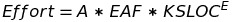
\includegraphics[width=0.4\textwidth]{equationFM.png}}%
\vspace*{0cm}
\end{figure}
\begin{figure}[h]
\vspace*{\fill}
\noindent\makebox[\textwidth]{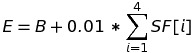
\includegraphics[width=0.35\textwidth]{E.png}}%
\vspace*{0cm}
\end{figure}

where the parameters are:\\
\begin{tabular}{ | l| }
\hline
A=2.94\\
B=0.91\\
EAF = Product of all cost drivers = 1.4336\\
E = Exponent derived from the scale drivers=0.91+0.01*13.57=1.0457\\
LowBoundKSLOC=8.134\\
HighBoundKSLOC=11.122\\
\hline
\end{tabular}\\\\
 Thus for the lower bound of the KSLOC was obtained:
 \begin{figure}[h]
\noindent\makebox[\textwidth]{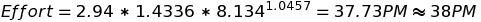
\includegraphics[width=0.7\textwidth]{ef1.png}}%
\end{figure}
and for the high bound of the KSLOC:
\begin{figure}[!h]
\noindent\makebox[\textwidth]{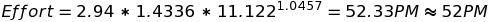
\includegraphics[width=0.7\textwidth]{ef2.png}}%
\end{figure}

\subsubsection{Schedule Estimation}
In terms of the schedule the following formulas will be need:
\begin{figure}[!h]
\noindent\makebox[\textwidth]{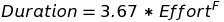
\includegraphics[width=0.4\textwidth]{schedule.png}}%
\end{figure}

\begin{figure}[!h]
\noindent\makebox[\textwidth]{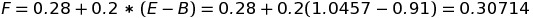
\includegraphics[width=0.95\textwidth]{F.png}}%
\end{figure}
The schedule considering the lower boud is:\\
\begin{figure}[!h]
\noindent\makebox[\textwidth]{
\includegraphics[width=0.75\textwidth]{durationLow.png}}%
\end{figure}\\
and the schedule considering the higher bound is:
\begin{figure}[!h]
\noindent\makebox[\textwidth]{
\includegraphics[width=0.75\textwidth]{durationHigh.png}}%
\end{figure}

\newpage
\section{Project Plan Schedule}
This section illustrate a high level view of the organization of the project schedule, showing the main phases of the production process. Should it be implemented, more detailed schedules for each of the phases and each of the sprints organized inside them will be defined during the project for better internal organization.\par
Due to the size of the Schedule Graph we separated in 4 different sections, RASD, DD, Development and Deployment.
\newline \par
\begin{figure}[h]
\centering
\vspace*{\fill}
\noindent\makebox[\textwidth]{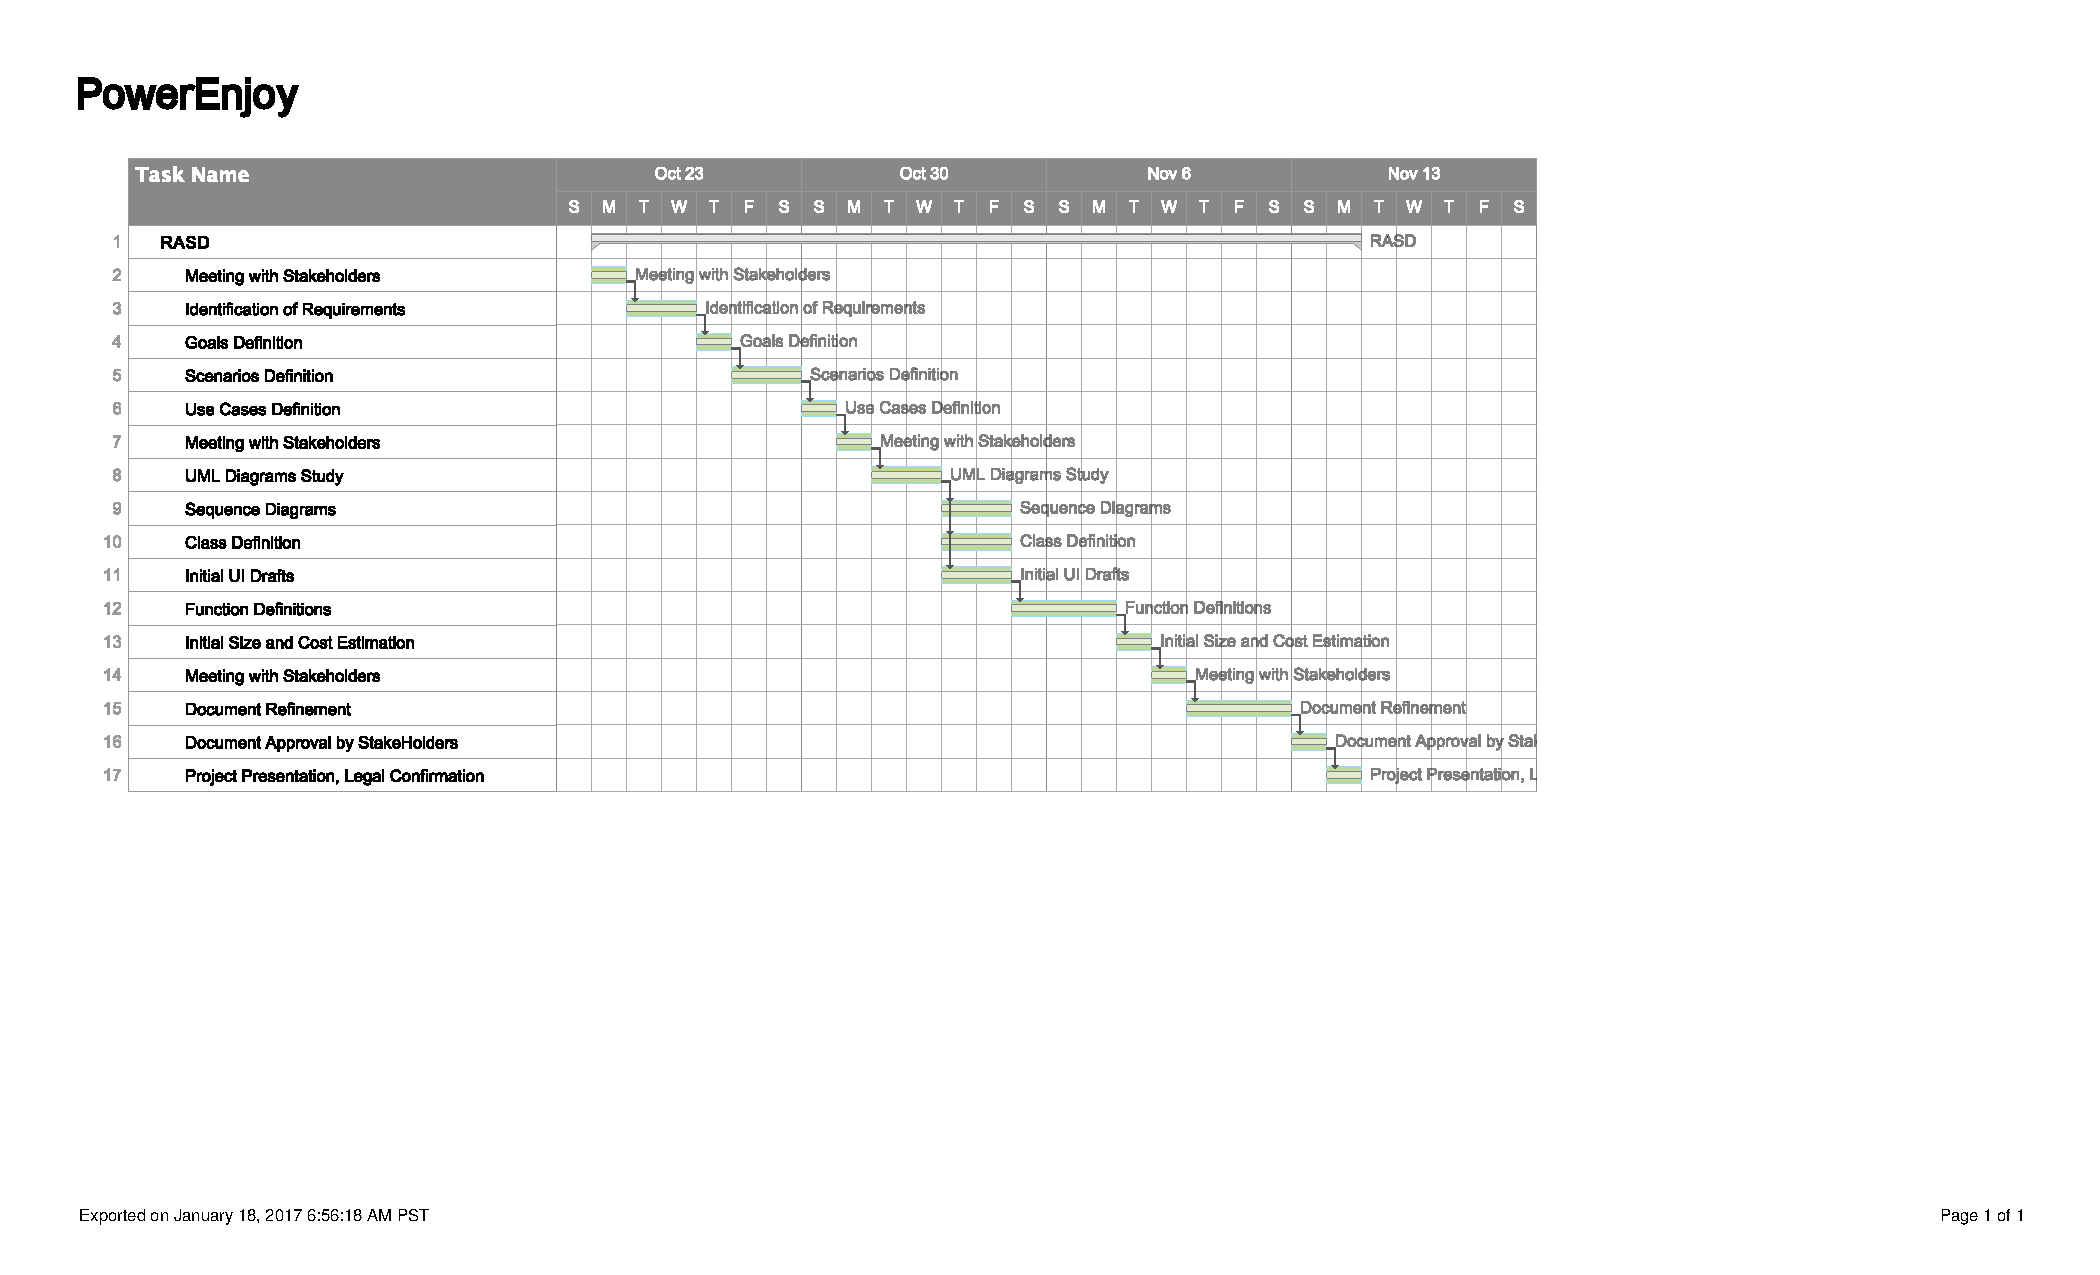
\includegraphics[width=1.5\textwidth]{RASD_Schedule.png}}%
\vspace*{0cm}
\end{figure}
\begin{figure}[h]
\centering
\vspace*{\fill}
\noindent\makebox[\textwidth]{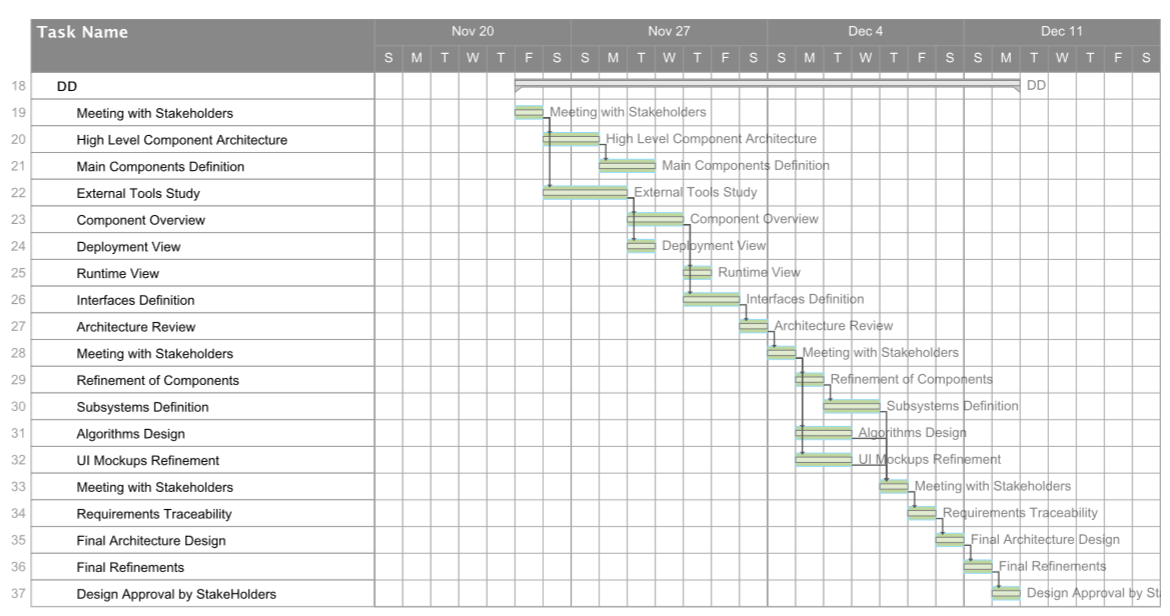
\includegraphics[width=1.42\textwidth]{DD_Schedule.png}}%
\vspace*{0cm}
\end{figure}
\begin{figure}[h]
\centering
\vspace*{\fill}
\noindent\makebox[\textwidth]{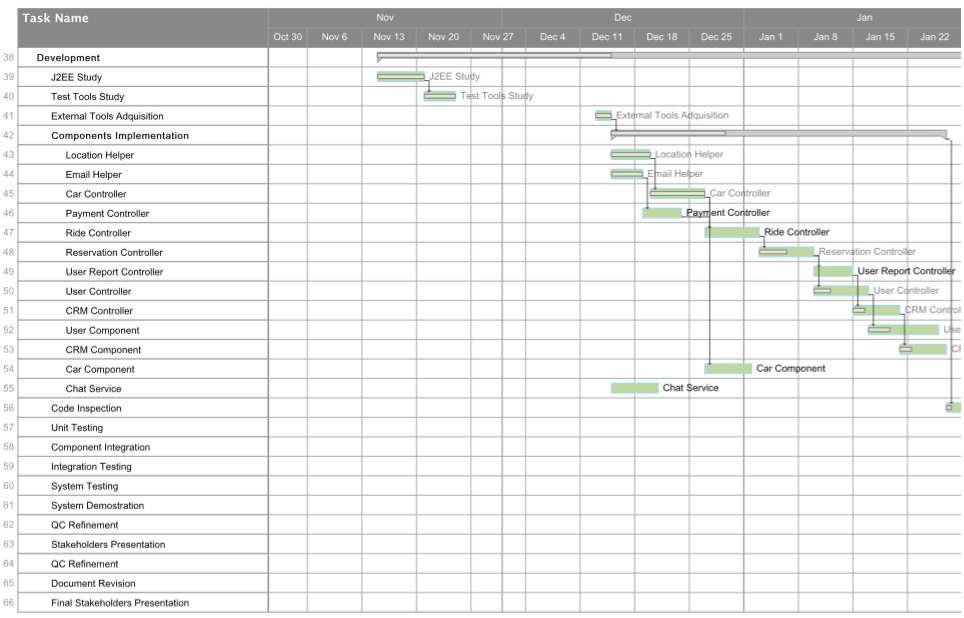
\includegraphics[width=1.42\textwidth]{Dev_Schedule1.png}}%
\vspace*{0.5cm}
\end{figure}
\begin{figure}[h]
\centering
\vspace*{\fill}
\noindent\makebox[\textwidth]{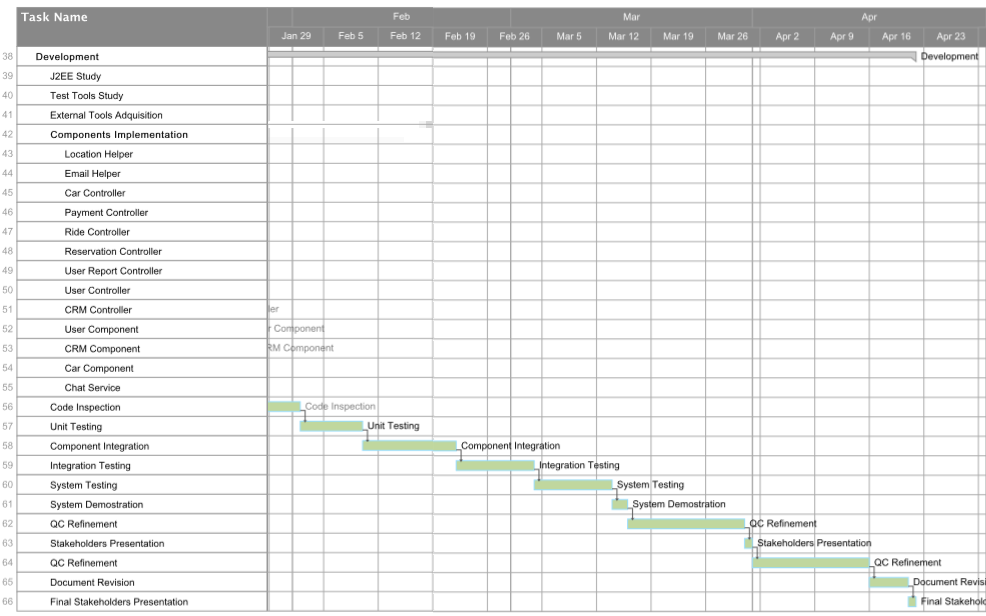
\includegraphics[width=1.5\textwidth]{Dev_Schedule2.png}}%
\vspace*{0.5cm}
\end{figure}
\begin{figure}[h]
\centering
\vspace*{\fill}
\noindent\makebox[\textwidth]{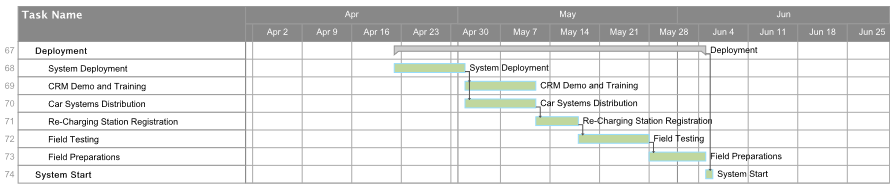
\includegraphics[width=1.5\textwidth]{Deployment_Schedule.png}}%
\vspace*{0.5cm}
\end{figure}

\section{Resource Allocation}
In this part of the document, it is defined the division of the tasks exposed in the previous section, according to each member of the team. \newline
Some general guidelines, that were specified in other parts of the project, were followed. As an example, no resource is single handed responsible for an entire task, in order to avoid missing deadlines in case someone is absent. Also, there are points where one member is allocated to two or more tasks while another is managing only one, this is not due individual capacities, but to the level of responsibility each has with the specific task. \newline
For better presentation, the section is divided in a chronological order for each team member. 
 

\begin{figure}[h]
\centering
\vspace*{\fill}
\noindent\makebox[\textwidth]{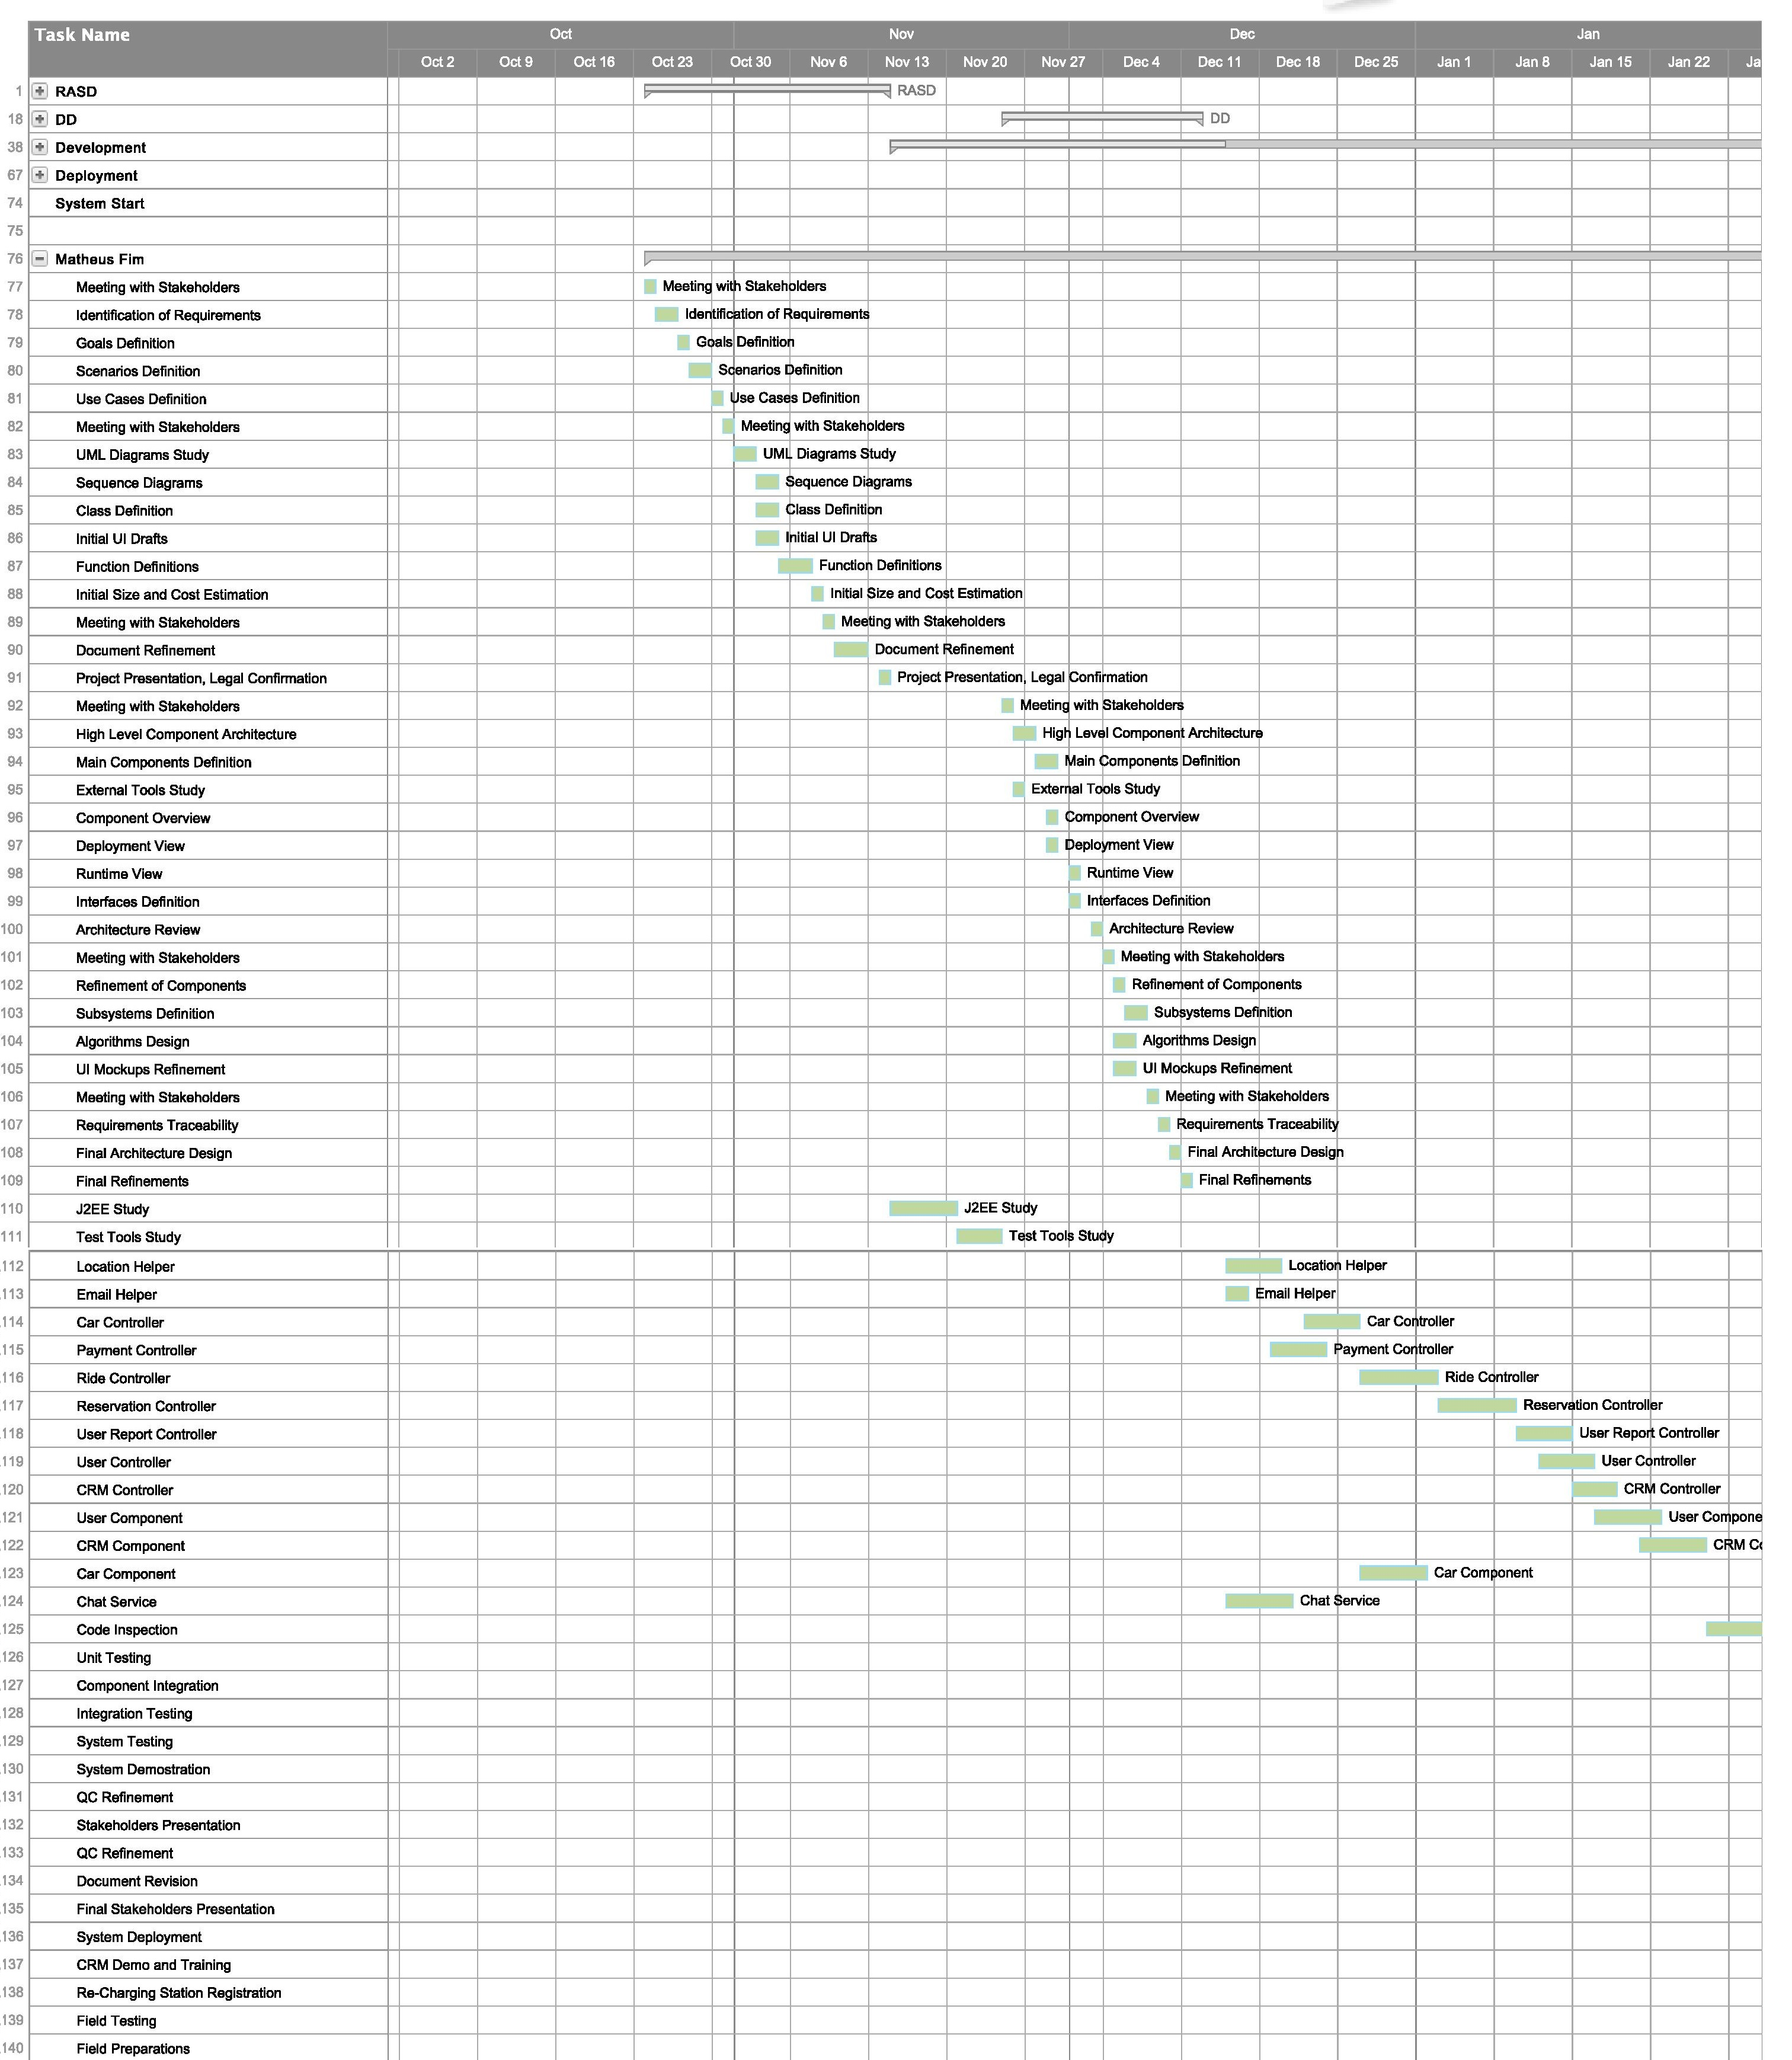
\includegraphics[width=1\textwidth]{m11.jpg}}%
\vspace*{0cm}
\end{figure}
\begin{figure}[h]
\centering
\vspace*{\fill}
\noindent\makebox[\textwidth]{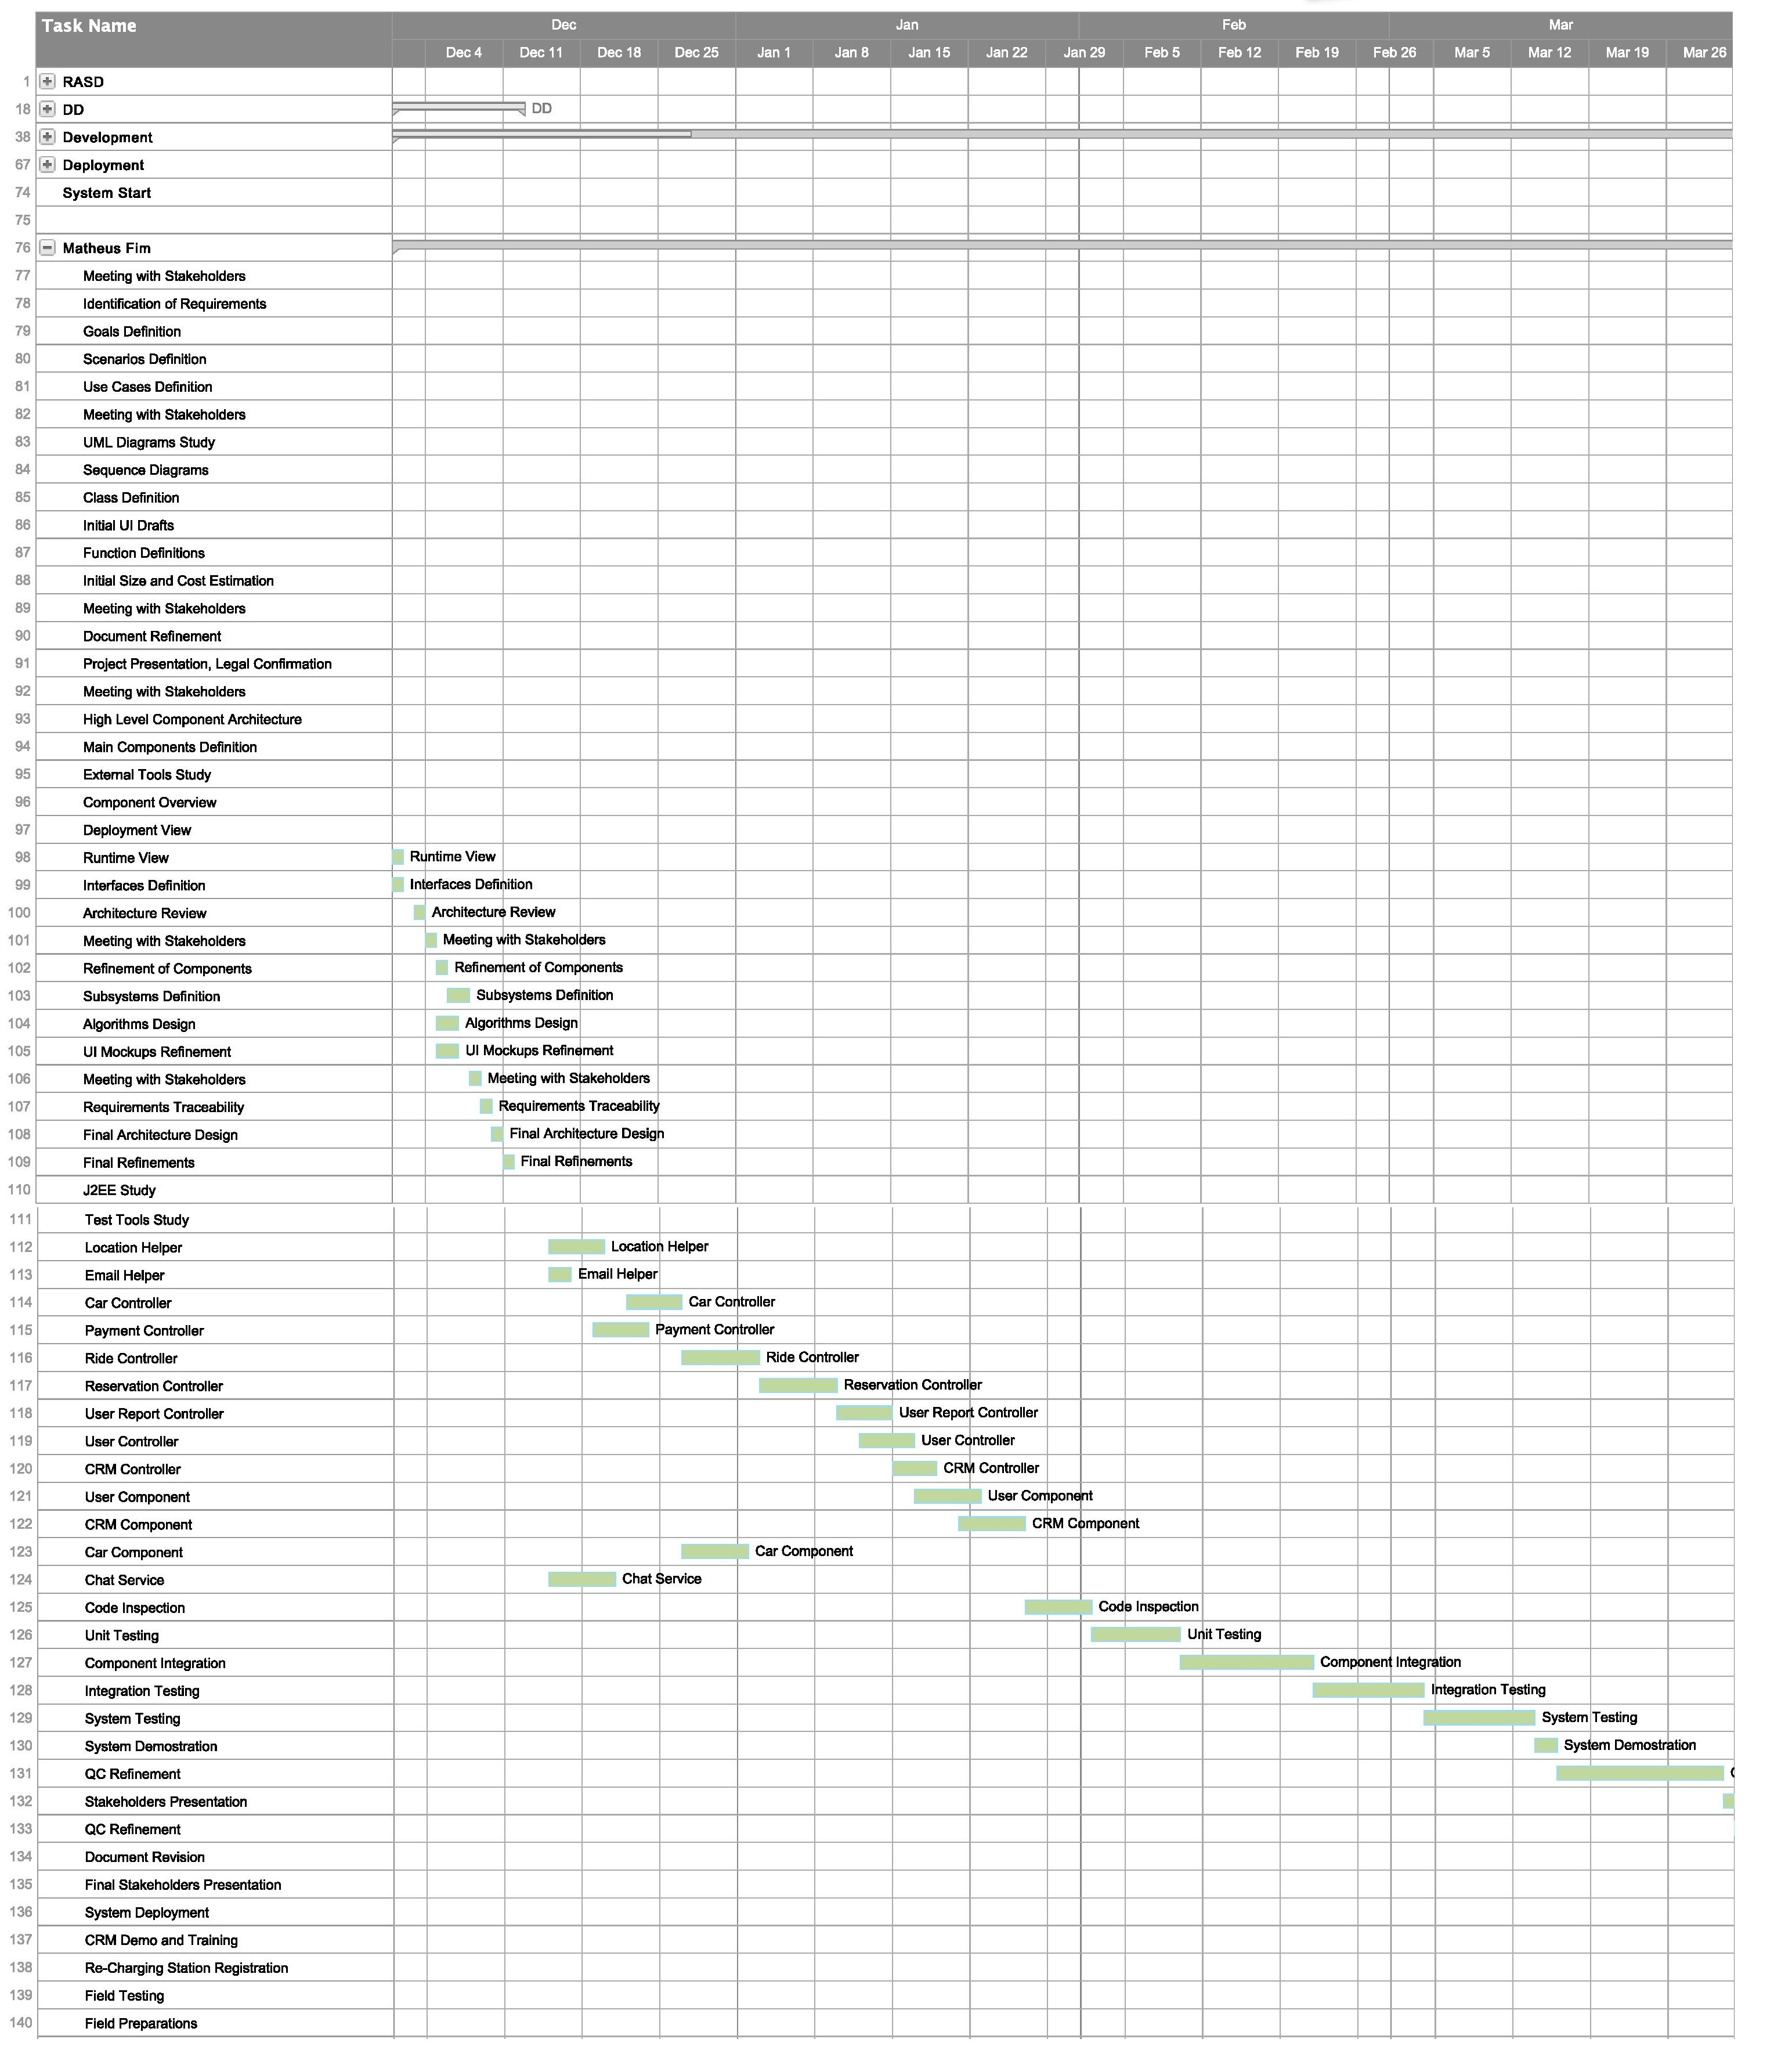
\includegraphics[width=1.2\textwidth]{m12.jpg}}%
\vspace*{0cm}
\end{figure}
\begin{figure}[h]
\centering
\vspace*{\fill}
\noindent\makebox[\textwidth]{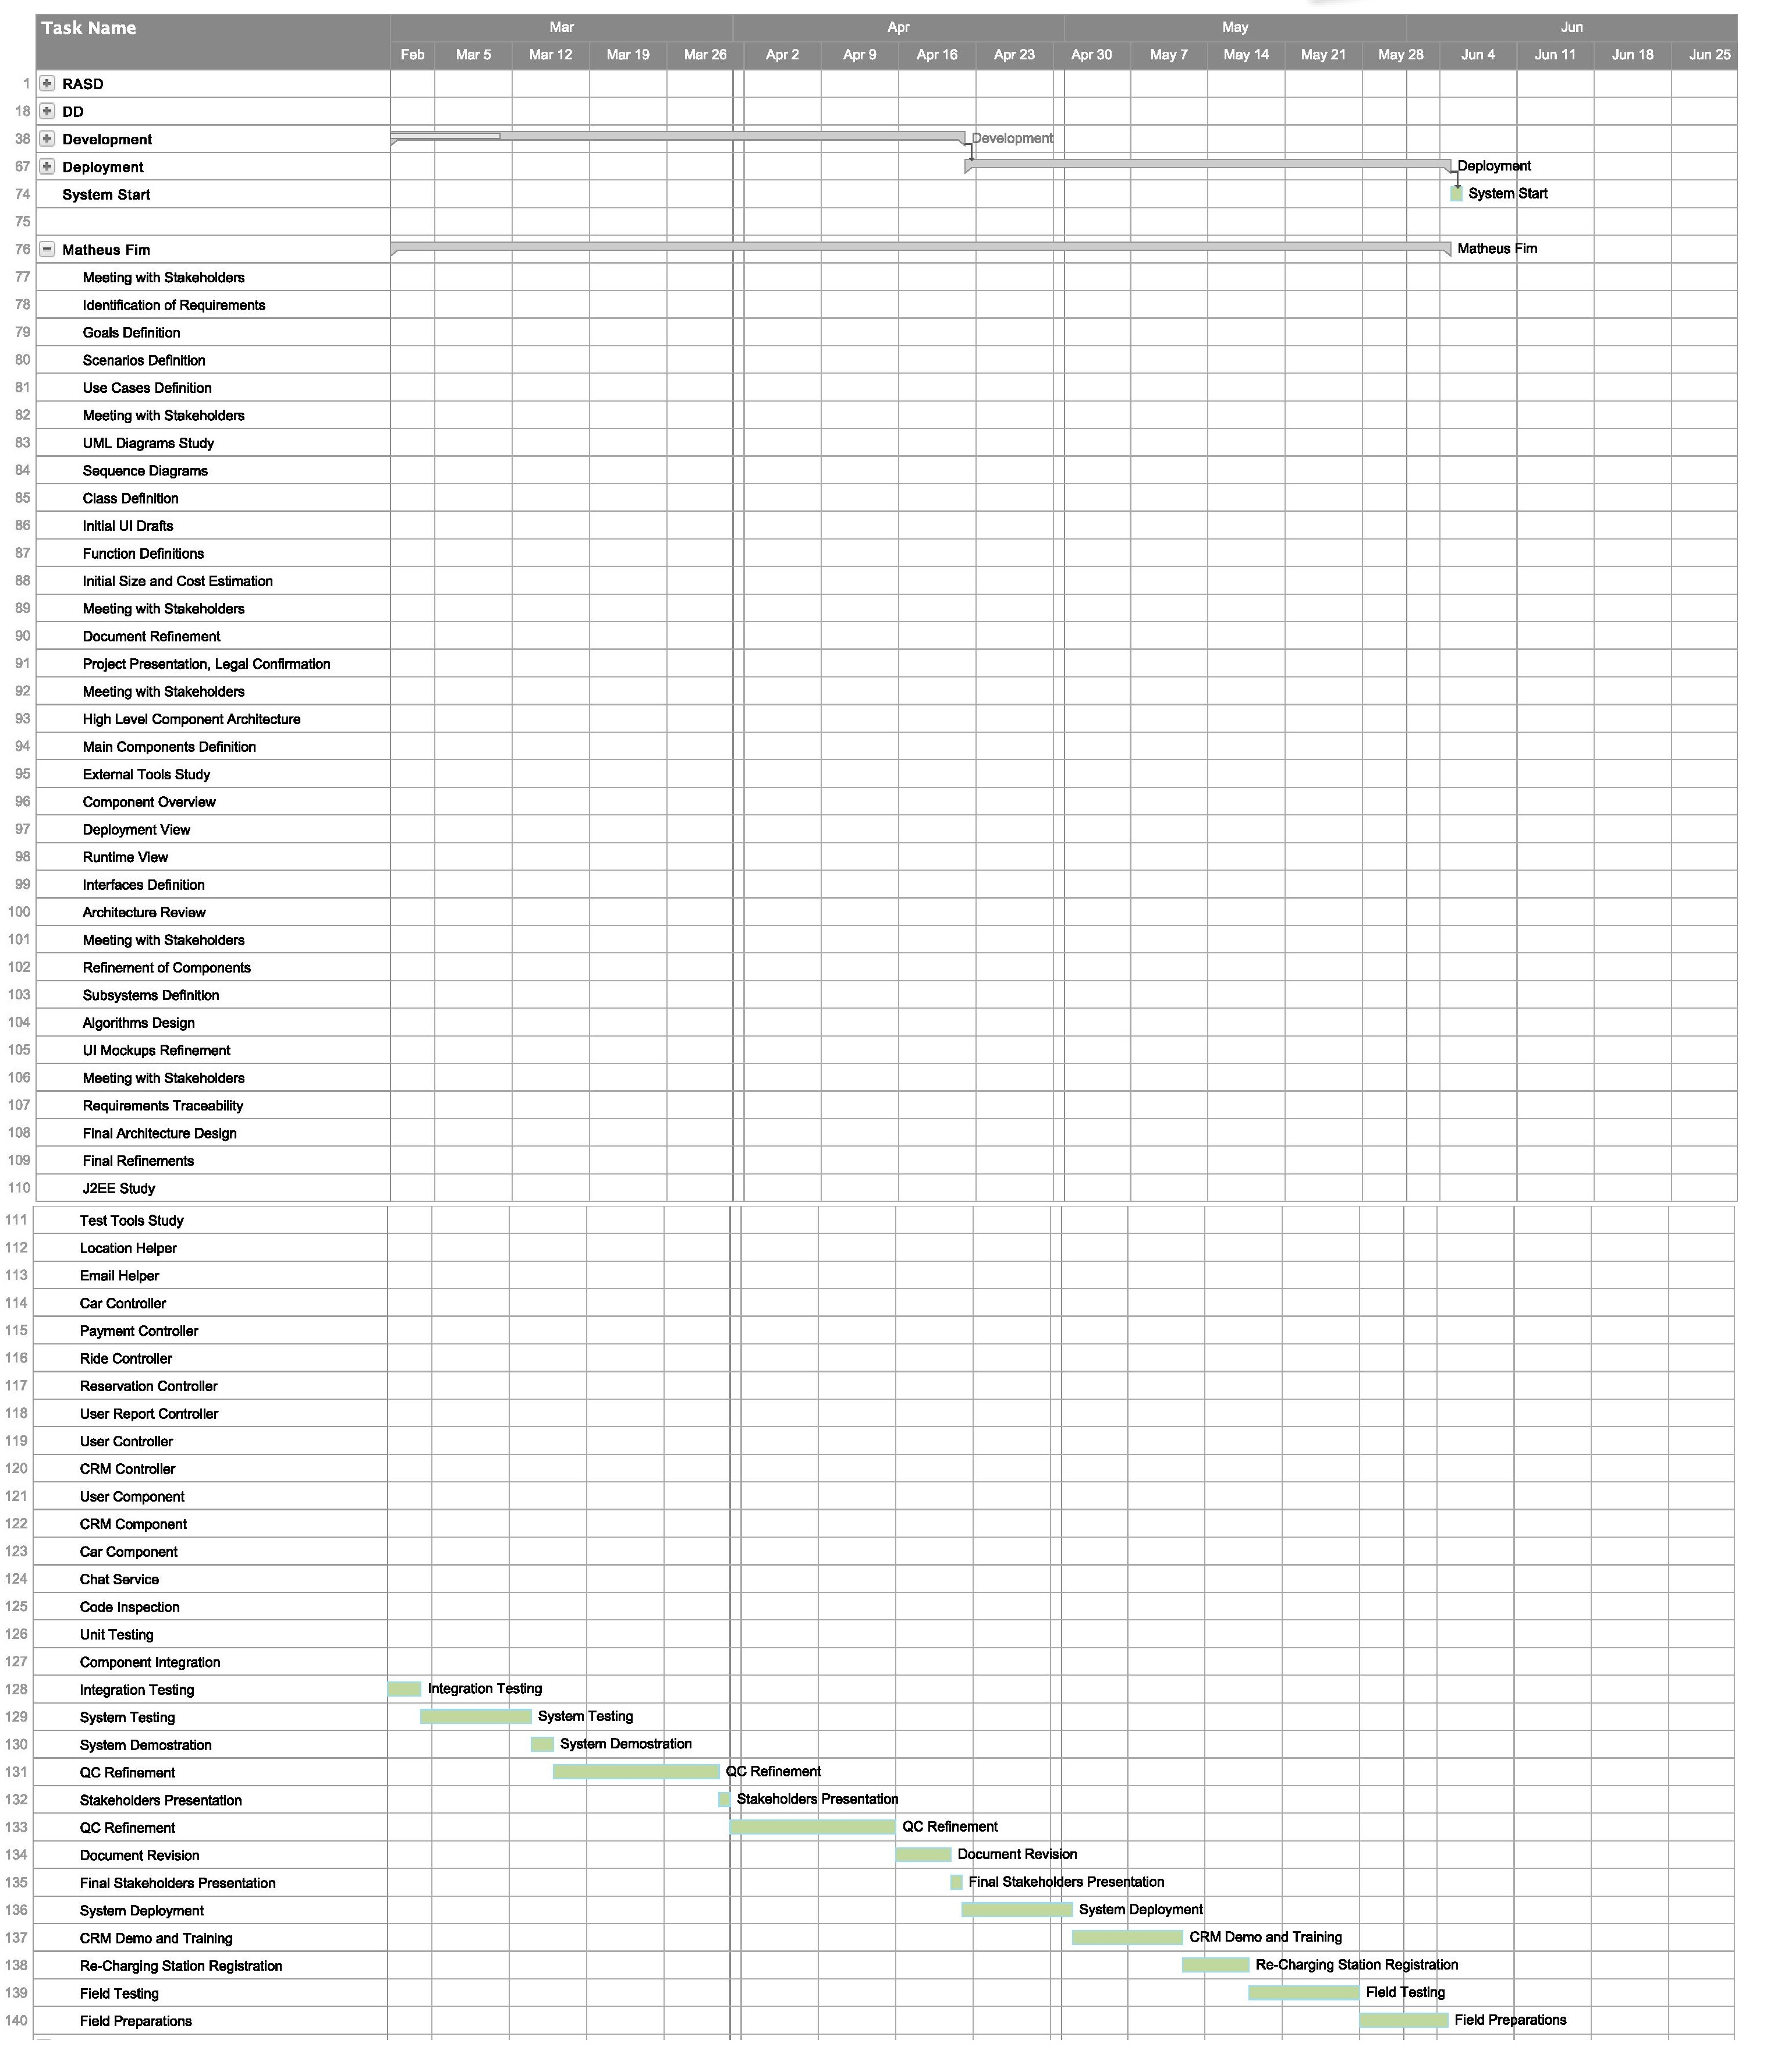
\includegraphics[width=1.2\textwidth]{m13.jpg}}%
\vspace*{0cm}
\end{figure}


\begin{figure}[h]
\centering
\vspace*{\fill}
\noindent\makebox[\textwidth]{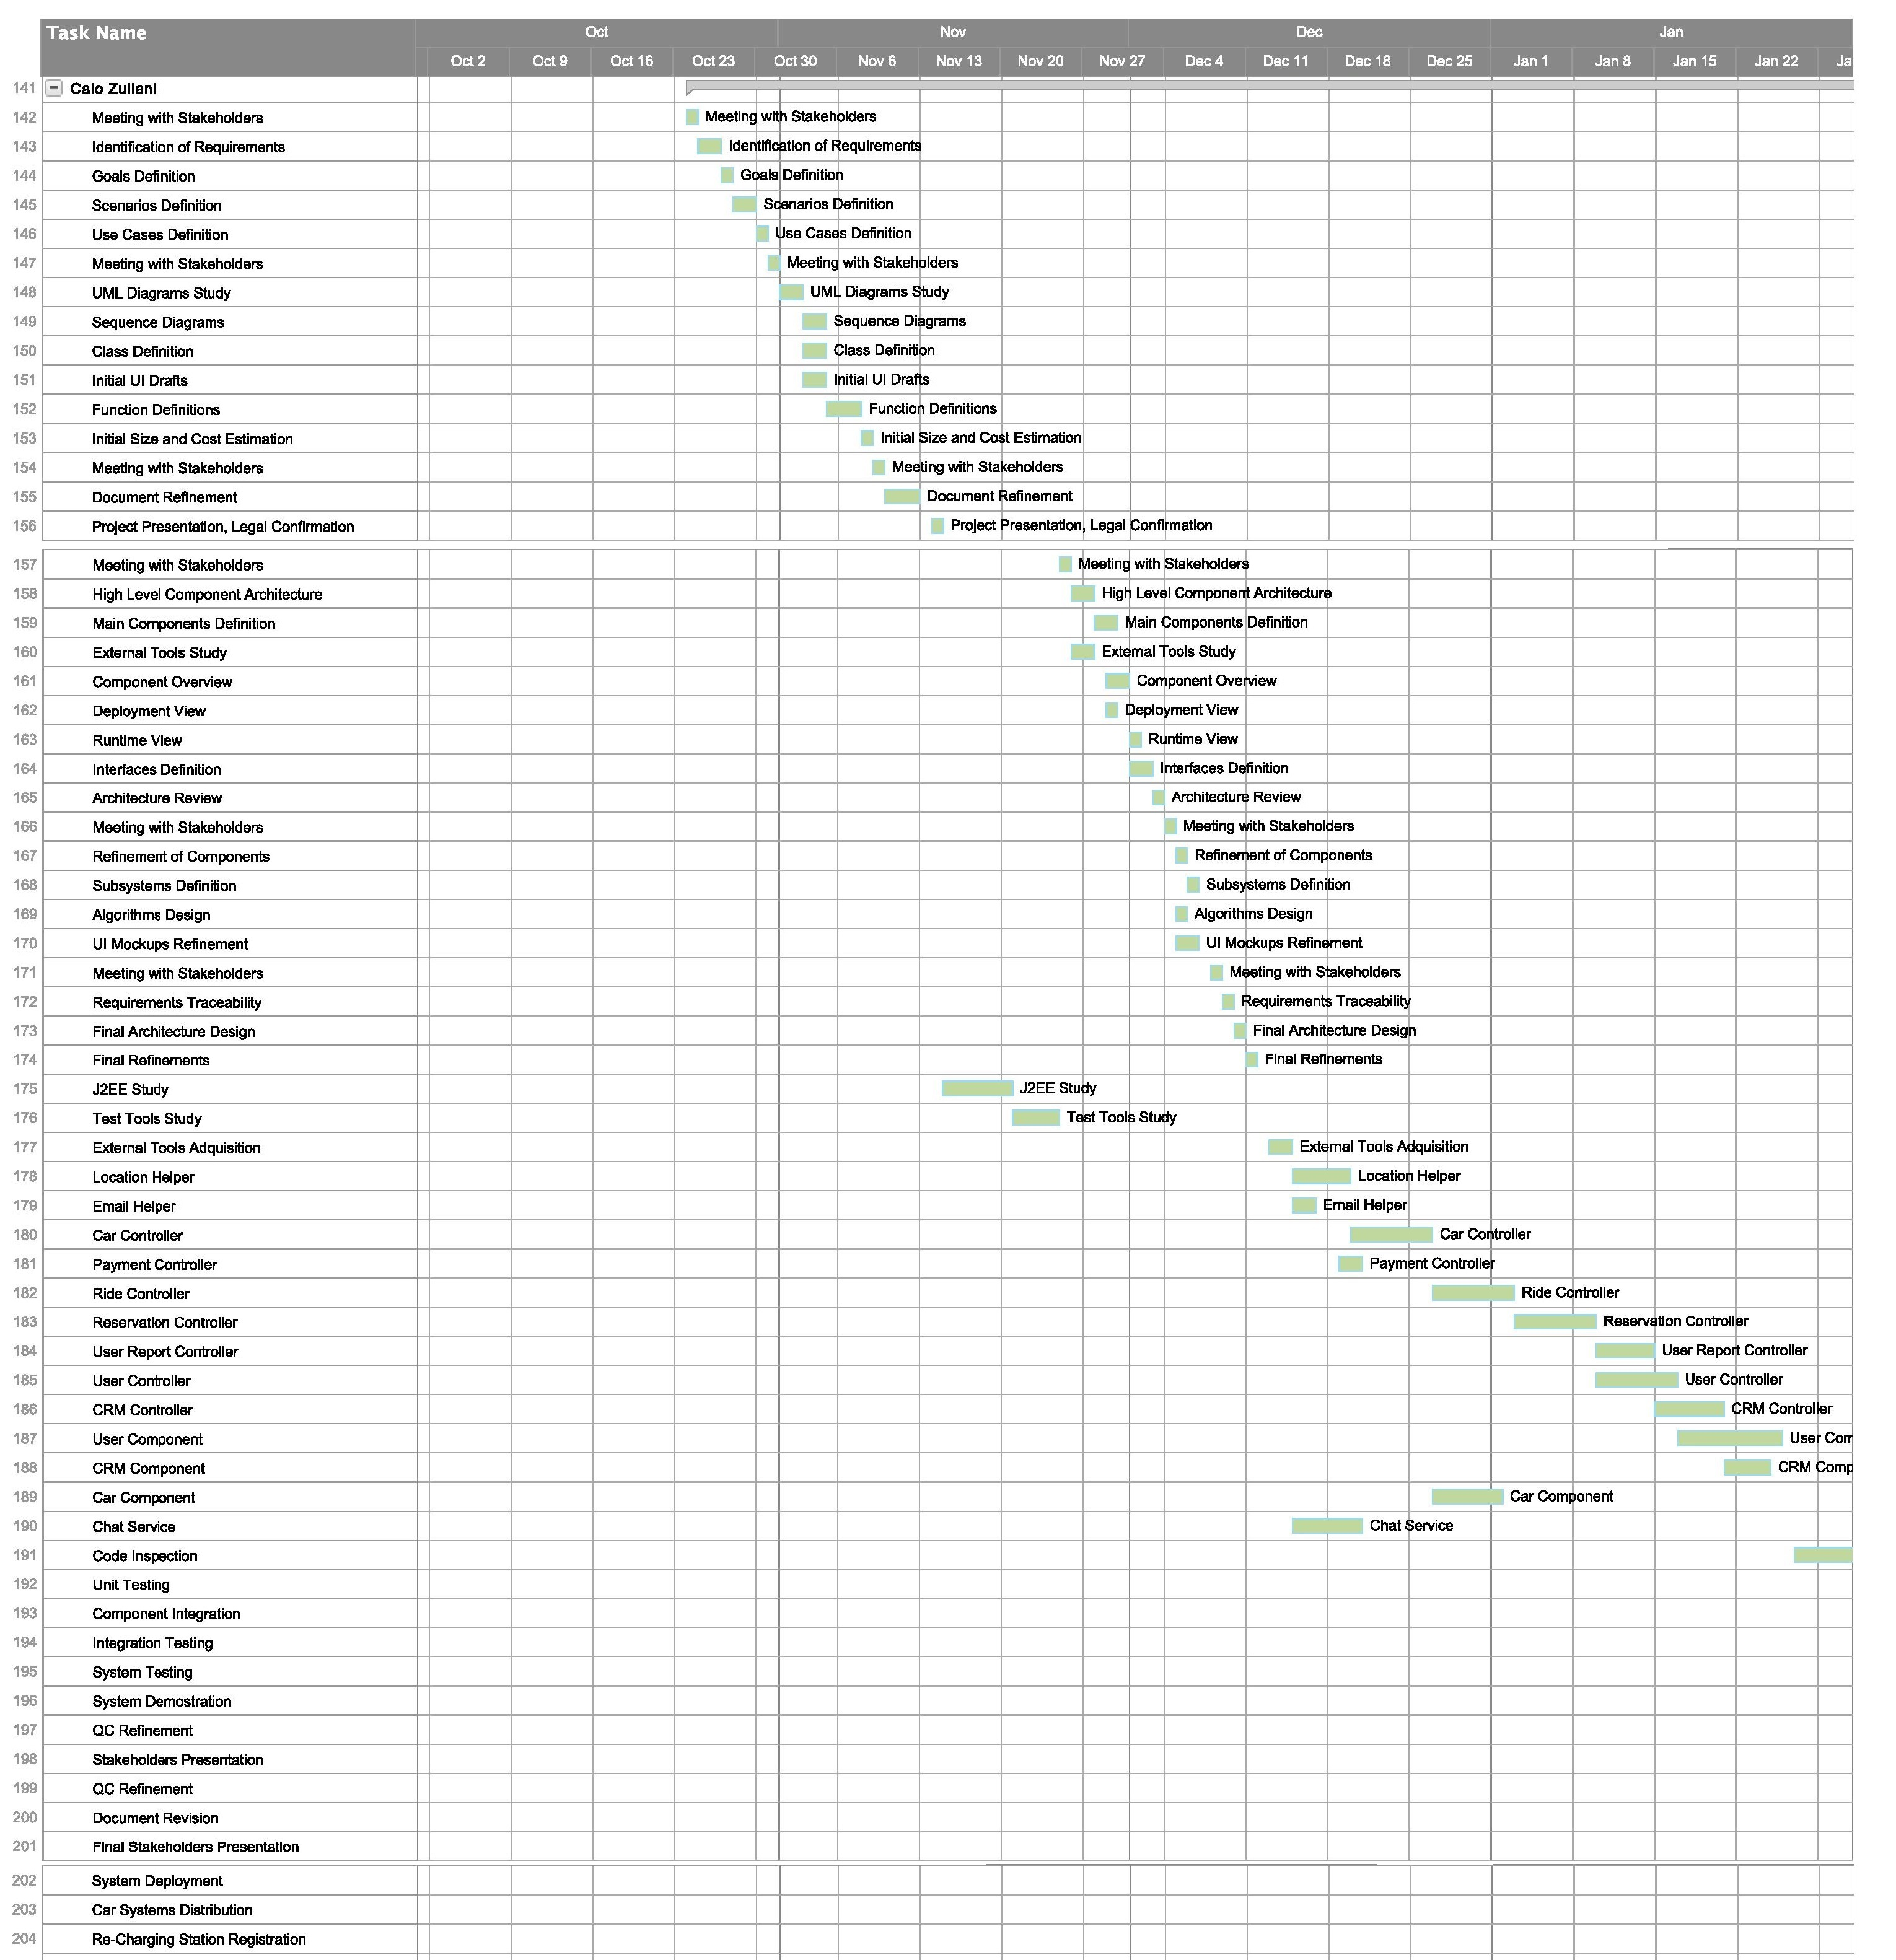
\includegraphics[width=1.2\textwidth]{c11.jpg}}%
\vspace*{0cm}
\end{figure}
\begin{figure}[h]
\centering
\vspace*{\fill}
\noindent\makebox[\textwidth]{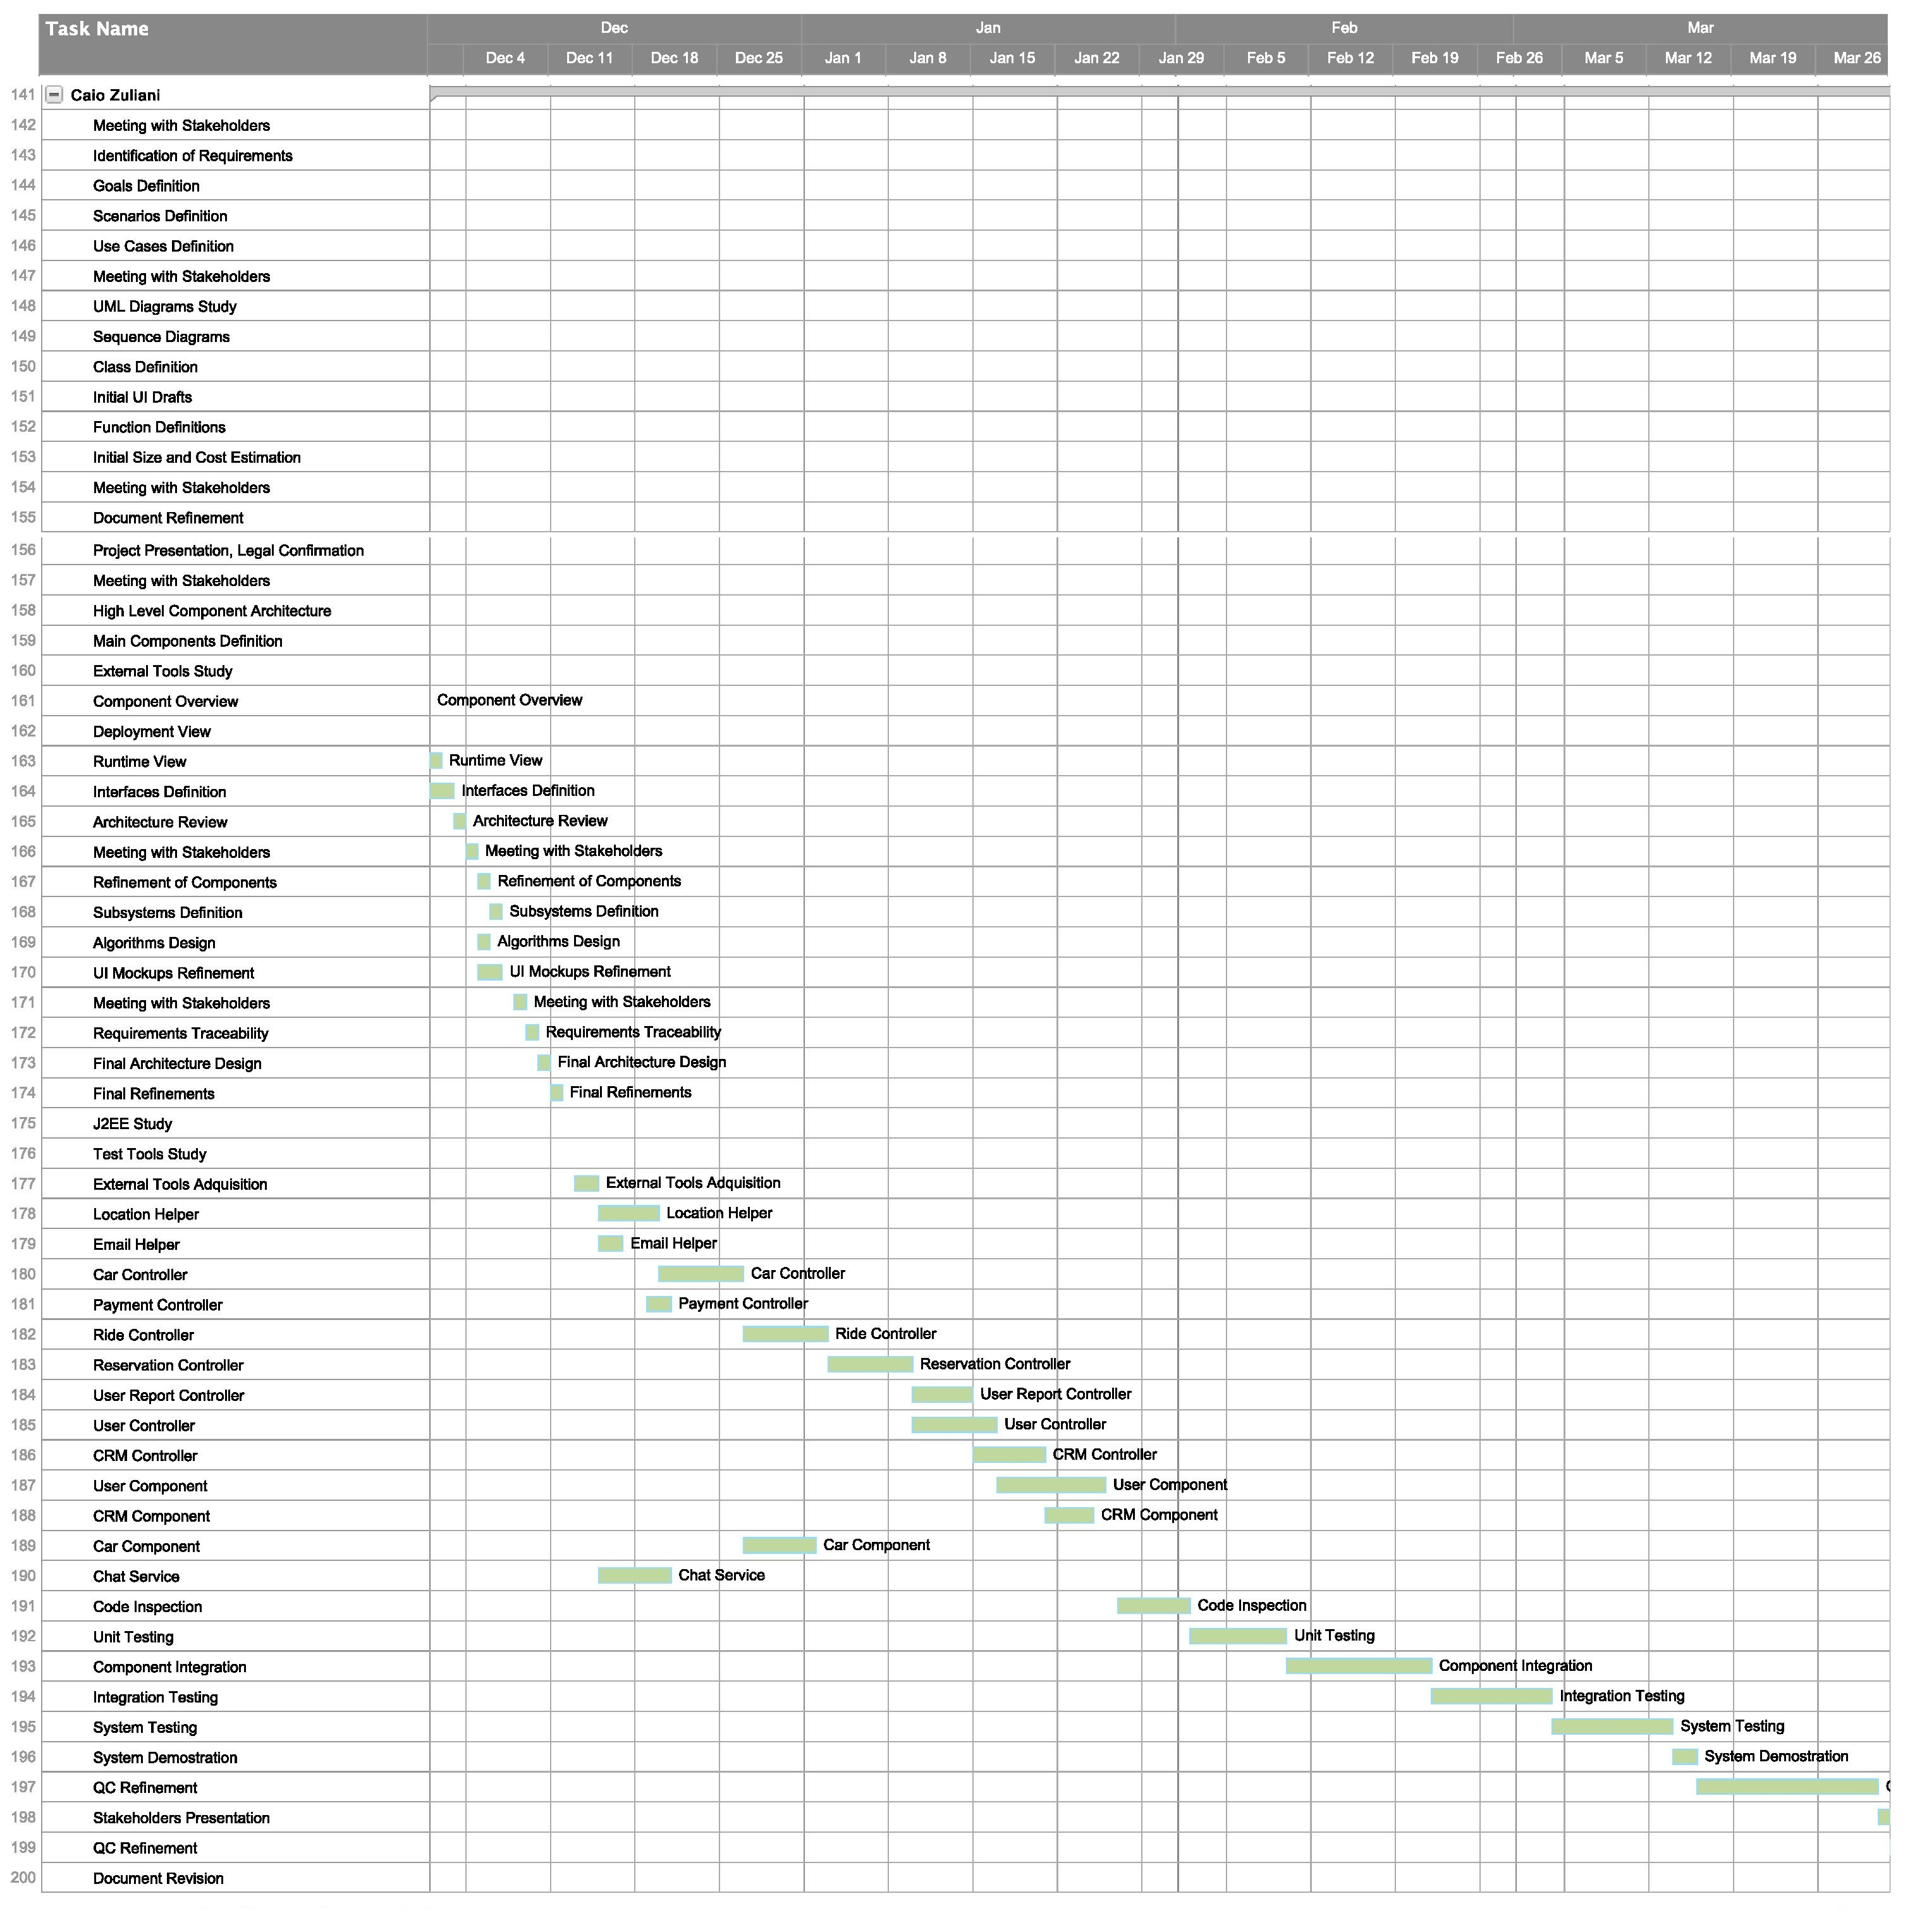
\includegraphics[width=1.2\textwidth]{c12.jpg}}%
\vspace*{0cm}
\end{figure}
\begin{figure}[h]
\centering
\vspace*{\fill}
\noindent\makebox[\textwidth]{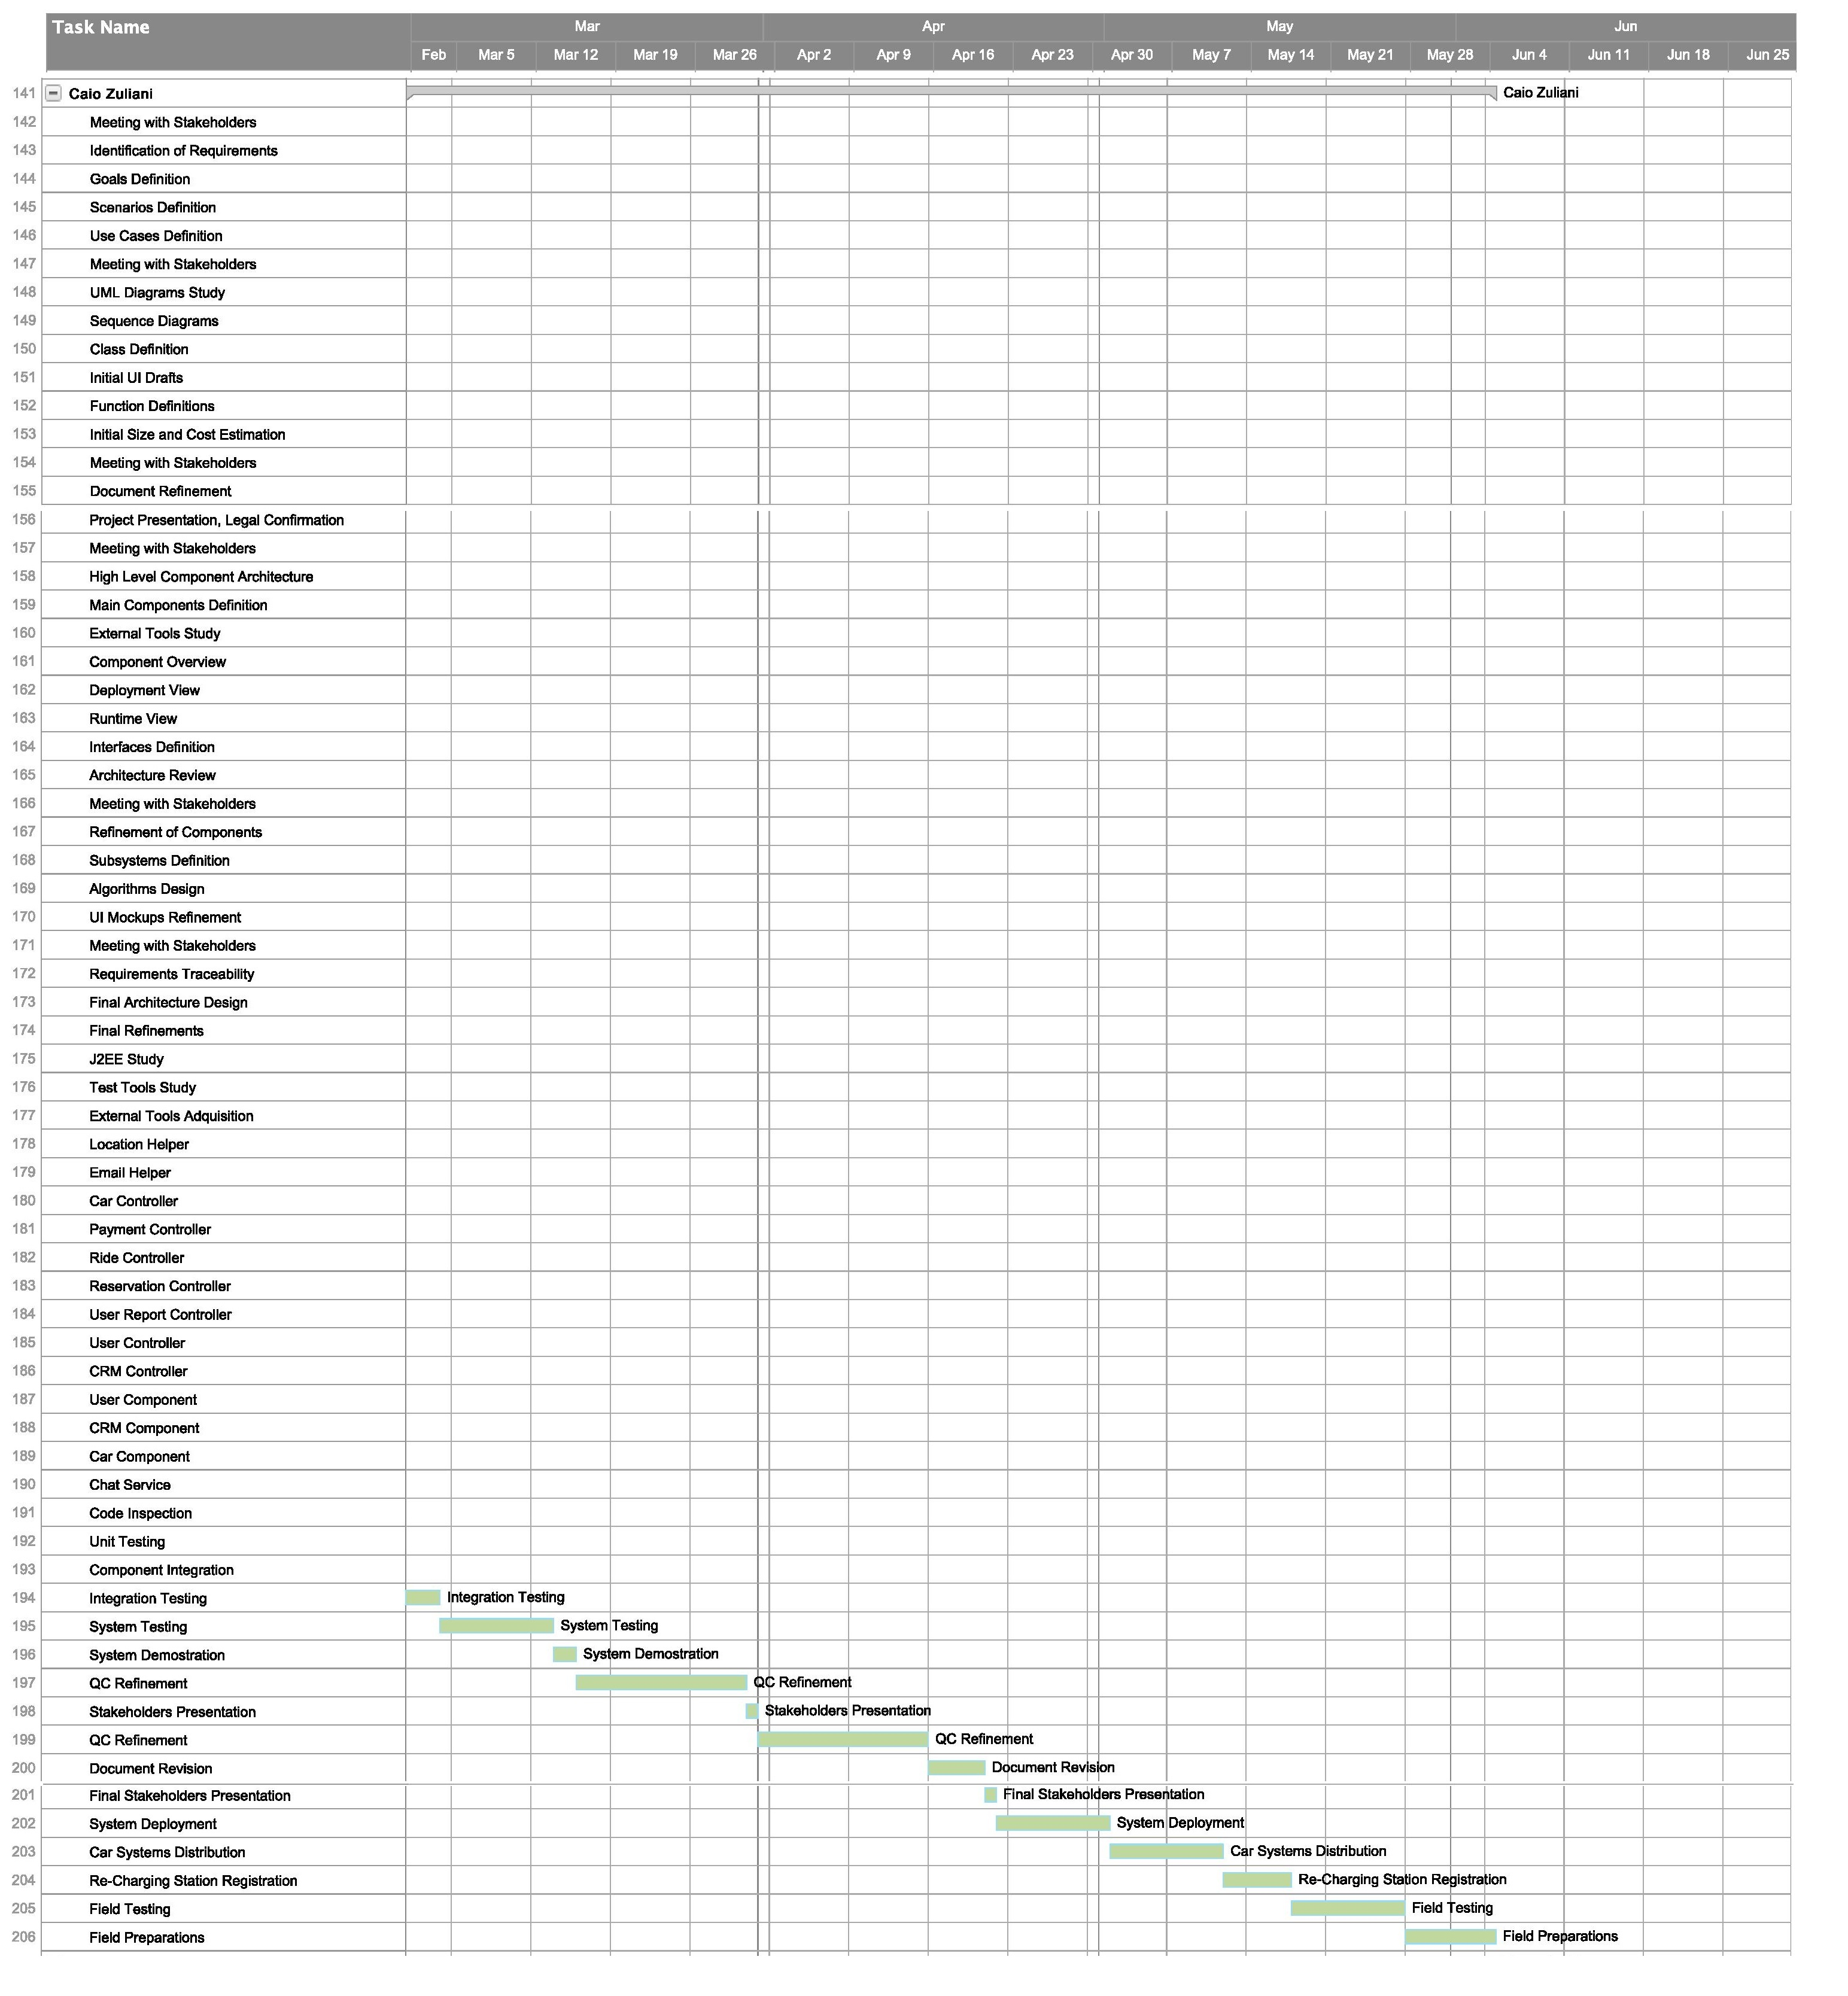
\includegraphics[width=1.2\textwidth]{c13.jpg}}%
\vspace*{0cm}
\end{figure}


\begin{figure}[h]
\centering
\vspace*{\fill}
\noindent\makebox[\textwidth]{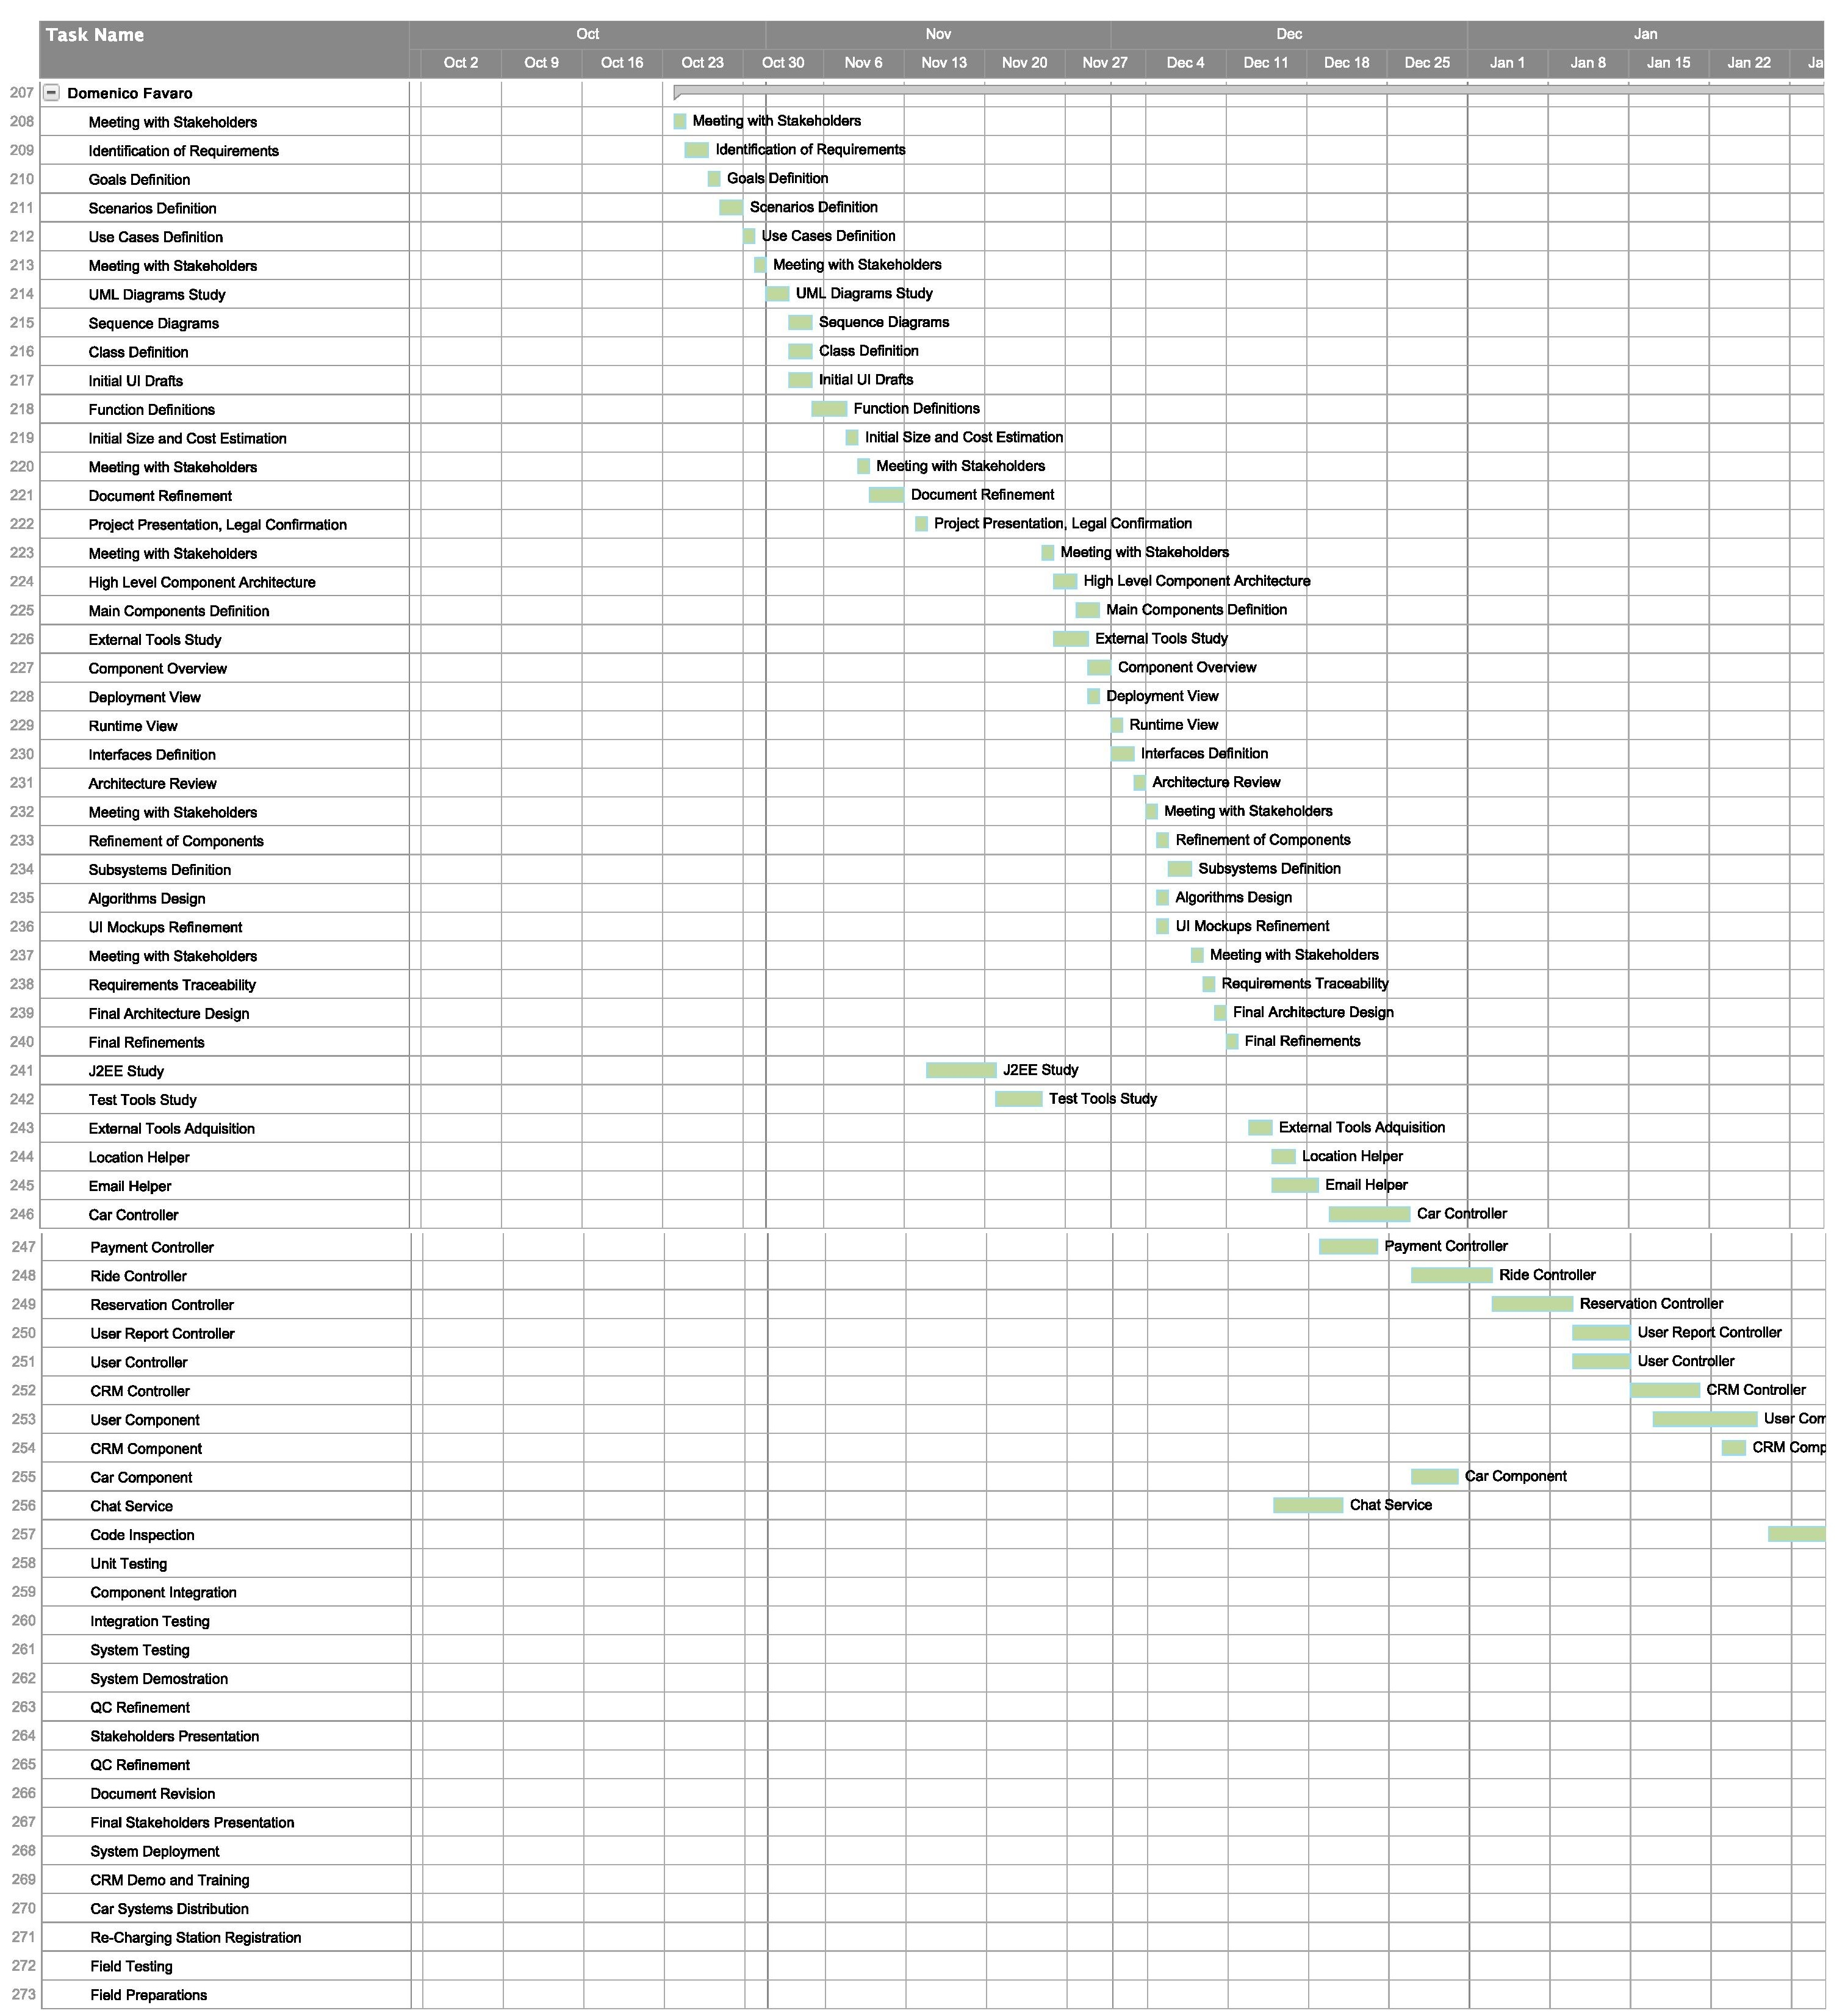
\includegraphics[width=1.2\textwidth]{d11.jpg}}%
\vspace*{0cm}
\end{figure}
\begin{figure}[h]
\centering
\vspace*{\fill}
\noindent\makebox[\textwidth]{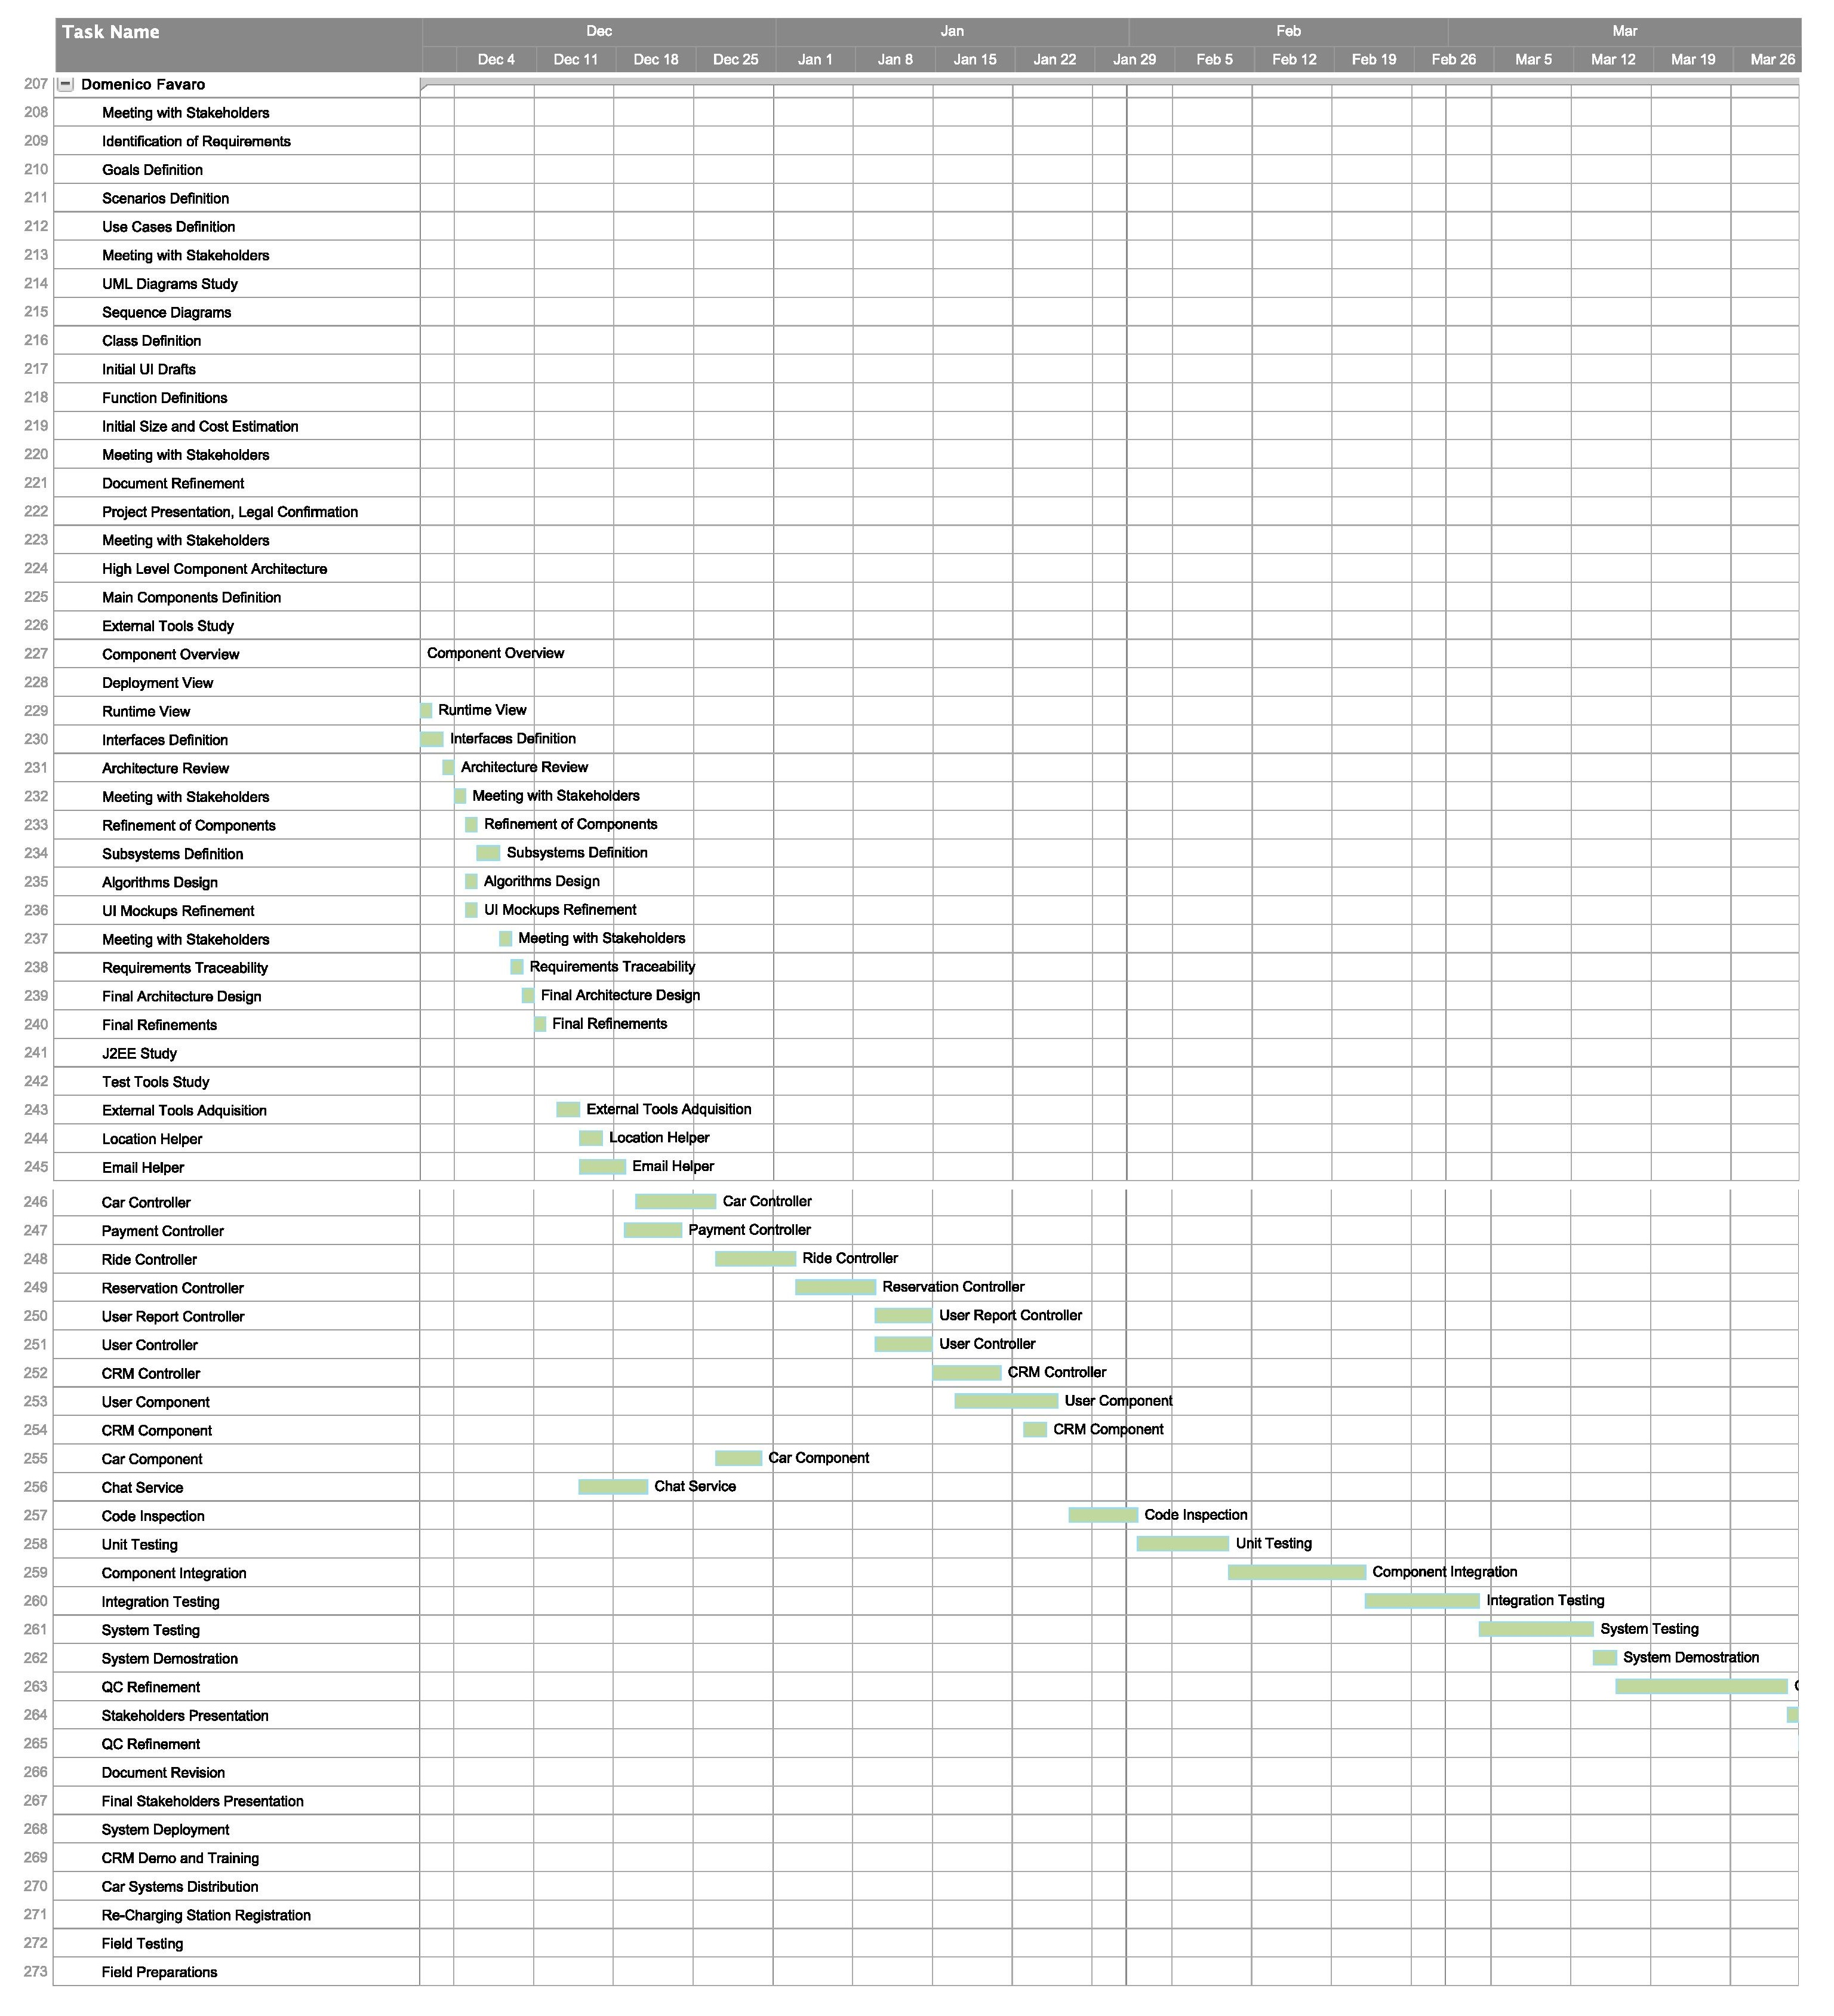
\includegraphics[width=1.2\textwidth]{d12.jpg}}%
\vspace*{0cm}
\end{figure}
\begin{figure}[h]
\centering
\vspace*{\fill}
\noindent\makebox[\textwidth]{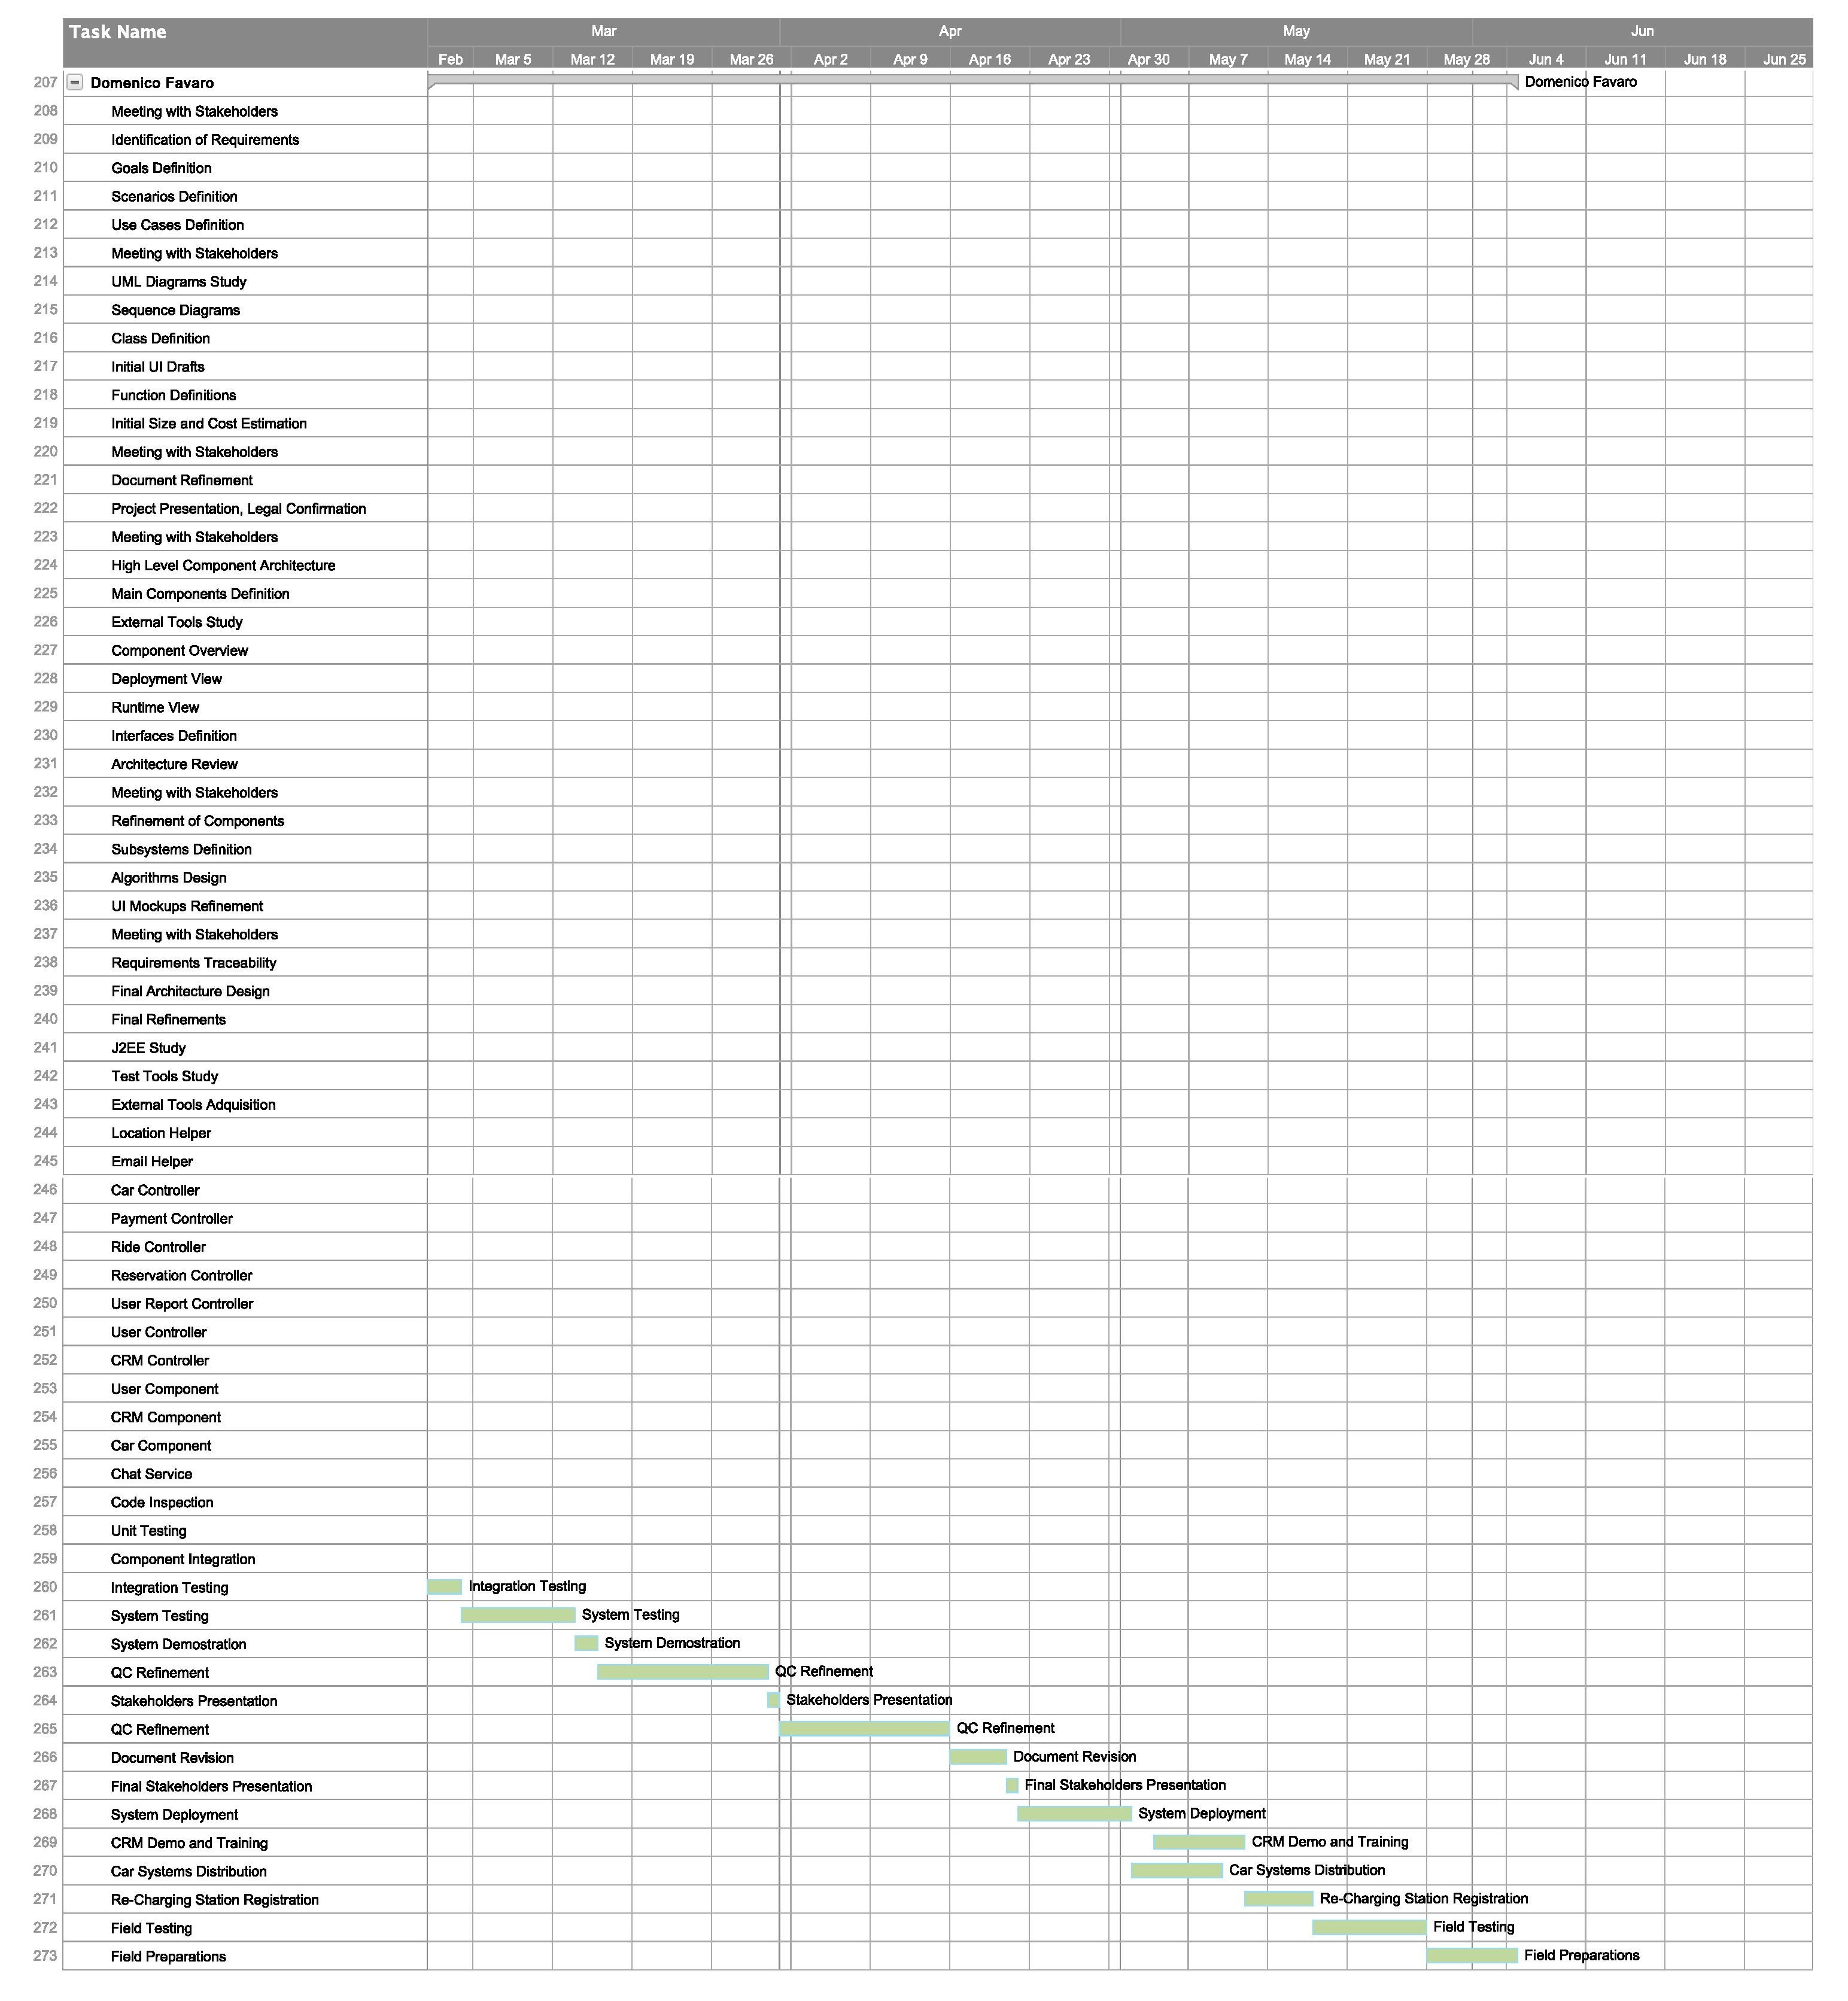
\includegraphics[width=1.2\textwidth]{d13.jpg}}%
\vspace*{0cm}
\end{figure}
\section{Risk Management}

This section aims at defining at an early stage what are the risks regarding this project, and by doing so, define what are the indicators of a risk materializing itself and the actions that should be taken. The risk management is a continuous process. Therefore, the following are guidelines that should be upgraded as the project progresses. 

A common risks computer softwares face are that the delivered product is not in total accordance with the vision the client had, and thus does not fully attend the functionalities proposed. Or it may happen that the users and CRM staff are not pleased with the final version, resulting in some resistance to use the product and bad public acceptance. This type of risks are managed by involving both the client and the users into early stages of development. The client should participate in the requirement analysis, design, and be presented with constant reports and demonstrations of new functionalities, while the users need to be brought to test functionalities and interfaces every time it is possible, especially before they are final versions. The same is the case for the CRM team, apart from bringing them closer to the development, it is important to also provide training on how to use the final system, to ensure a low resistance to the software and increase the quality of the deployed service.  

A predictable risk is a turnover in the client situation, demanding the decrease of resources or the project to be completed in less time. Such scenario may arise for different reason, as example, a competitor company announces that will release a similar service before PowerEnjoy or a financial crisis is causing the client to invest less money than expected. Those are completely different problems, but the overall guidelines are the same: promote a negotiation with the client, explaining the consequences of this action. If, however, it is really necessary to do such change, establish a plan of incremental deployments, being the first one on the date set or using the money provided with limited functionalities, and make incremental deliveries as time or money become available.   

There are risks that represent greater problems as they cannot have clear contingency plans beforehand, such are the cases of legislation changes regarding the car sharing service in Italy.  New laws concerning the parking spots and other traffic rules can cause significantly changes in the product. And, although this scenario is hard to predict, such changes don’t come unnoticed, and by maintaining a good relationship with the city hall is possible to be aware with enough antecedence to adapt the service. 

The deployed system, inevitably will depend on external solutions, as the cloud infrastructure and the mapping service. For the first, it is necessary to do a complete market research before choosing the company that will provide the service, some key points are: a clear contract, defining what are the changes that can happen in the cloud infrastructure and binding them to send a notice before doing so; the structure used should be as generic as possible, predicting that in case of having to migrate, the damage is minimized; the line between price and quality here should be pending to the quality side. As for the second, the used solution is well-known and widely accepted, Google maps. For this reason, instability or changes in the service are not a high concern, nonetheless, in case it does not meet the company needs anymore, a replacement should already be kept in background, with some preliminary tests on migration. 

Also the database, payment and e-mail are factor of risks, they have a serious effects but low probability and are easily fixed due to the fact they are relatively standardized. Backup routines should be established and followed rigorously, with redundant copies in different medias. Still regarding data loss,  the source code needs to be included in the backups and the developers should be constantly reminded to keep the quality of the GIT repository, following the specifications for the commits.  

Some internal problems may be summarized as the unavailability of a staff member. To ensure that no functionality is left undone, no member is single handed responsible for a specific part, or in other words, the work distributions overlaps themselves.  But, as this is a small team, it may result in overload of work for the remaining members. This may be a difficult point to solve, as the period of absence in unsure, one of the management technique adopted that helps this and almost most issues in the development phase is to include extra time in the ending of major tasks.      

A final predicted risk, is the failure of the screen inside the car, as it is a hardware piece it is subjected multiple malfunctions. As for the quality of the product, extensive testing with different hardwares was predicted in the testing phase, so, in case of the hardware proves to be insufficient to the needs of the system, there are other tested options. And for punctual failures, the company is advised to keep spare screens in stock for a fast change. Of course, the later a problem is detected here, the more expensive is to fix it. As an example, if on development it is discovered that the first option for the screen breaks easily after little use, there are only a few to be replaced, but if the system was already deployed, this may result in huge losses for the company. 

The above consideration (the later a risk presents itself the more expensive it is to fix it) tends to be true for most cases, hence it is why is crucial to keep reviewing the contingency plans and monitoring the signals that a risk, predicted or non predicted, may arise. 


\newpage
\section{Effort Spent}
\begin{tabular}{ | c | c | c | c | }
\hline
	\textbf {Date} & \textbf {Domenico} & \textbf {Caio} & \textbf {Matheus} \\ \hline
	15/01/17& 2h & 2h & 2h  \\ \hline
	16/01/17& - & - & - \\ \hline
	17/01/17& 4h & - & - \\ \hline
	18/01/17& 4h & - & - \\ \hline
	19/01/17& - & 6h & - \\ \hline
	20/01/17& - & 6h & 1h \\ \hline
	21/01/17& - & 1h & 6h \\ \hline
<<<<<<< HEAD
	22/01/17& 2h & - & 2h \\ \hline
=======
	22/01/17& - & 1h & - \\ \hline
>>>>>>> 08ad59922da3744c8014679ca92f1a4d6f7e8f4b
\end{tabular}
\newpage

\section{Changelog}
As the project and design decisions may change during the development this document is also prone to change.
We'll document every version in this part.
\begin{itemize}
\item \textbf {Version 1.1:} 22/01/2017
\end{itemize}
\end{document}
